\documentclass[11pt]{beamer}

\usetheme{Madrid}

\usepackage{listings}
\usepackage{color}
\usepackage{float}
\usepackage{graphicx,subfigure}
\usepackage{algorithm2e}
\usepackage{tikz}
\usepackage[framemethod=TikZ]{mdframed}
\usepackage{breqn}
\usetikzlibrary{shapes,shadows,arrows}

%\newcommand{\red}{\color{red}}
%\newcommand{\blue}{\color{blue}}
%\newcommand{\blue}{\color{green}}



\begin{document}

\defverbatim[colored]\lstI{
\begin{lstlisting}[language=C++,basicstyle=\ttfamily,keywordstyle=\color{red}]
function Solve(BLOCK){
	Iterate psi using Gauss-Seidel
	Solve omega using TDMA
	Calculate u and v
}
do{
	SetBoundaryConditions
	Solve(BLOCK1)
	Solve(BLOCK2)
	Solve(BLOCK3)
	Solve(BLOCK4)
	Solve(BLOCK5)
	Calculate error
}while error>10^-5
\end{lstlisting}
}

\defverbatim[colored]\lstII{
\begin{lstlisting}[language=C++,basicstyle=\ttfamily,keywordstyle=\color{red}]
__global__ void matrix_mul(...){
	...
	[GPU (Parallel) code]
	...
}

void main(){
	...
	[CPU (serial) code]
	[Copy CPU variables to GPU]
	matrix_mul<<<dimGrid, dimBlock>>>(...)
	[Copy GPU variables to CPU ]
	[CPU (serial) code]
	...
}

\end{lstlisting}
}

\defverbatim[colored]\lstIII{
\begin{lstlisting}[language=C++,basicstyle=\ttfamily,keywordstyle=\color{red}]
__global__ void kernelFunc(...)
{
    int idx = blockIdx.x * blockDim.x + threadIdx.x;
    if(idx < size)
    	{
        	...
        }
}
\end{lstlisting}
}



\title{PARALLEL COMPUTATION OF SOME INCOMPRESSIBLE VISCOUS FLOW PROBLEM BY BLOCK DECOMPOSITION}
\author{Sizil Krishna}
\institute{Indian Institute of Technology Guwahati}
\maketitle

\begin{frame}{Fluid Dynamics}{Introduction}
Generally the steps to tackle Computer Simulation is as follows.
\begin{itemize}
\item Fetch governing equations.
\item Discritize equations to apply computation.
\item Compute / Simulate problem using relevant algorithms. 
\end{itemize}

We'll be computing fluid flow in some standard problem domains following the above mentioned steps.
\end{frame}


\begin{frame}{Fluid Dynamics}{Introduction}
Governing equations are,
\linebreak
\linebreak
\textbf{Navier-Stokes} equation is given as,
\begin{equation} \label{eqn1}
\rho\left(\frac{\partial V}{\partial t} + V. \bigtriangledown V\right) =- \bigtriangledown p +  \mu\bigtriangledown^2 V  
\end{equation}\\

\textbf{Continuity equation} is given as,
\begin{equation}
\frac{\partial \rho}{\partial t} + \triangledown (\rho  V) = 0
\end{equation}
where, $\rho$ is density, $V = u\hat{i}, v\hat{j}, w\hat{k}$ is velocity vector, $\mu$ is the (constant) dynamic viscosity, $p$ is pressure and $\bigtriangledown = \left( \frac{\partial}{\partial x} , \frac{\partial}{\partial y} , \frac{\partial}{\partial z} \right)$.
\end{frame}

\begin{frame}{Fluid Dynamics}{Introduction}
For incompressible fluid flow in 2-D, the continuity equation can be rewritten as,
\begin{eqnarray}
\rho = constant \nonumber\\
\frac{\partial u}{\partial x} + \frac{\partial v}{\partial y} = 0 
\end{eqnarray} 

where $u$ and $v$ are the velocities in the x and y coordinate directions, respectively. Now we can introduce Stream function $\psi$ for a two dimensional flow as ,
\begin{eqnarray}
u=\frac{\partial \psi}{\partial y}, \hspace{1cm} v=-\frac{\partial \psi}{\partial x}
\end{eqnarray}
Where Stream function represents trajectories of particles in a steady flow.
\end{frame}


\begin{frame}{Fluid Dynamics}{Introduction}

The vorticity of a flow is a pseudovector field $\omega$, equal to the curl (rotational) of its velocity field $V$.

It describes the local spinning motion of a fluid near some point.
Thus vorticity can be written as,
\begin{eqnarray}
\omega &=& \bigtriangledown \times V 
= \begin{bmatrix}
\frac{\partial}{\partial x} & \frac{\partial}{\partial y} \\
u & v 
\end{bmatrix} \nonumber\\
&=& \frac{\partial v}{\partial x} - \frac{\partial u}{\partial y} \nonumber\\
&=& - \frac{\partial^{2} \psi}{\partial x^{2}} - \frac{\partial^{2} \psi}{\partial y^{2}} \nonumber\\
&=& - \bigtriangledown ^{2} \psi \nonumber
\end{eqnarray}
Or,
\begin{equation}
\bigtriangledown ^{2} \psi = -\omega
\end{equation}
\end{frame}


\begin{frame}{Fluid Dynamics}{Introduction - Discritization}
\textbf{Discritization of equations}
\linebreak
\linebreak
\textbf{Finite-difference methods} are numerical methods for approximating the solutions to differential equations using finite difference equations to approximate derivatives. \linebreak
Discritization makes it easy to solve a equation using advanced computational iterators and solvers.

\begin{eqnarray} \label{eqn2} \nonumber
Forward-difference &:& f'(a) \approx \frac{f(a+h)-f(a)}{h} \nonumber\\
Backward-difference &:& f'(a) \approx \frac{f(a)-f(a-h)}{h}  \nonumber\\
Central-difference &:&  f'(a) \approx \frac{f(a+h)-f(a-h)}{2h} \nonumber
\end{eqnarray}
where $h$ being the gap between two consecutive points.
\end{frame}


\begin{frame}{Fluid Dynamics}{Introduction - Discritization}
\begin{figure}[hH]
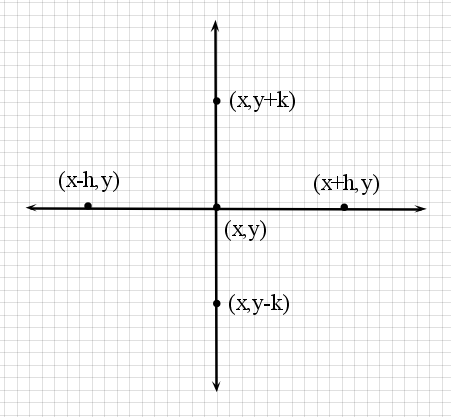
\includegraphics[width=0.3\textwidth]{images/1}
\end{figure}
Finite-difference scheme of a second order derivative can be given as,
\begin{equation}
f_{xy}(x,y) \approx \frac{ \begin{split} f(x+h,y+k) - f(x+h,y-k) \\
- f(x-h,y+k) + f(x-h,y-k) \end{split} }{4hk}
\end{equation}
where $h$ being the gap between two consecutive points in x direction and $k$ in y direction.
\end{frame}

\begin{frame}{Fluid Dynamics}{Introduction - Discritization}
\textbf{Steady State Flow}
\linebreak
Steady state flow means that no flow parameters (velocity, pressure etc ) depend on time. The time dependant terms in Navier-Stokes and continuity equations drop off. The governing equations are,
\begin{equation} \label{eqn25}
\frac{\partial \psi}{\partial y}.\frac{\partial \omega}{\partial x} - \frac{\partial \psi}{\partial x}.\frac{\partial \omega}{\partial y} = \frac{1}{Re}\left[\frac{\partial ^{2}\psi}{\partial x^{2}} + \frac{\partial ^{2}\psi}{\partial y^{2}}\right]
\end{equation}
where $Re$ is Reynolds number (constant introduced to make equations dimensionless). The discretized form of above equation is,
\begin{eqnarray} \label{spsi} 
\psi_{i,j} &=& \frac{\psi_{i+1,j} + \psi_{i-1,j} + \beta^{2}(\psi_{i,j+1} + \psi_{i,j-1}) + (\Delta x)^{2}\omega_{i,j}}{2(1+\beta^{2})} \\
\beta &=& \frac{\Delta x }{\Delta y} \nonumber
\end{eqnarray}
where, $\Delta x$ is grid size in $X$ direction and $\Delta y$ is grid size in $Y$ direction.
\end{frame}

\begin{frame}{Fluid Dynamics}{Introduction - Discritization}
\begin{figure}[hH]
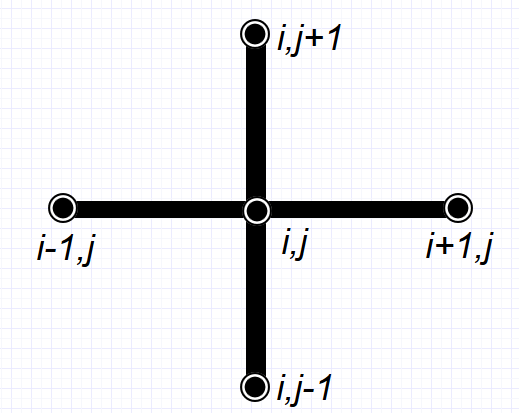
\includegraphics[width=0.3\textwidth]{images/2}
\end{figure}
\begin{equation} \label{somega}
\omega_{i,j} = \frac{ \begin{split} \omega_{i+1,j} + \omega_{i-1,j} + \beta ^{2}(\omega_{i,j+1} + \omega_{i,j-1}) -\\ \frac{1}{4}\beta Re(\omega_{i+1,j} - \omega_{i-1,j})(\psi_{i,j+1} - \psi_{i,j-1}) +\\
\frac{1}{4}\beta Re(\omega_{i,j+1} -   \omega_{i,j-1})(\psi_{i+1,j} - \psi_{i-1,j})\end{split}}{2(1+\beta^{2})}
\end{equation}
\end{frame}

\begin{frame}{Fluid Dynamics}{Introduction - Discritization}
\textbf{Unsteady State Flow}
\linebreak
Unsteady state means that various quantities like pressure, velocity etc depend on time. The Navier-Stokes equation in $\psi$-$\omega$ form is,
\begin{equation} \label{eqn222}
\frac{\partial \omega}{\partial t} + \frac{\partial \psi}{\partial y}\frac{\partial \omega}{\partial x} - \frac{\partial \psi}{\partial x}\frac{\partial \omega}{\partial y} = \frac{1}{Re}\left( \frac{\partial ^{2}\omega}{\partial x^{2}} + \frac{\partial ^{2}\omega}{\partial y^{2}} \right)
\end{equation}
Discretized forms are, 
\begin{eqnarray} \label{upsi}
\psi_{i,j} &=& \frac{\psi_{i+1,j} + \psi_{i-1,j} + \beta^{2}(\psi_{i,j+1} + \psi_{i,j-1}) + (\Delta x)^{2}\omega_{i,j}}{2(1+\beta^{2})} \\
\beta &=& \frac{\Delta x }{\Delta y} \nonumber
\end{eqnarray}
where, $\Delta x$ is grid size in $X$ direction and $\Delta y$ is grid size in $Y$ direction.
\end{frame}

\begin{frame}{Fluid Dynamics}{Introduction - Discritization}
$X Sweep :$
\begin{eqnarray}\label{uomega1}
\frac{\omega_{i,j}^{n+\frac{1}{2}} - \omega_{i,j}^{n}}{\frac{\Delta t}{2}} + v_{i,j}^{n} \left[\frac{\omega_{i,j+1}^{n} - \omega_{i,j-1}^{n}}{2h} \right] +  v_{i,j}^{n+\frac{1}{2}} \left[\frac{\omega_{i+1,j}^{n+\frac{1}{2}} - \omega_{i-1,j}^{n+\frac{1}{2}}}{2h} \right] = \nonumber \\
 \frac{1}{Re} \left[ \left[ \frac{\omega_{i+1,j}^{n+\frac{1}{2}} + \omega_{i-1,j}^{n+\frac{1}{2}} - 2\omega_{i,j}^{n+\frac{1}{2}}}{h^{2}} \right] +  \left[ \frac{\omega_{i,j+1}^{n} + \omega_{i,j-1}^{n} - 2\omega_{i,j}^{n}}{h^{2}} \right] \right] 
\end{eqnarray}
$Y Sweep :$
\begin{eqnarray}\label{uomega2}
\frac{\omega_{i,j}^{n+1} - \omega_{i,j}^{n+\frac{1}{2}}}{\frac{\Delta t}{2}} + v_{i,j}^{n+1} \left[\frac{\omega_{i,j+1}^{n+1} - \omega_{i,j-1}^{n+1}}{2h} \right] +  v_{i,j}^{n+\frac{1}{2}} \left[\frac{\omega_{i+1,j}^{n+\frac{1}{2}} - \omega_{i-1,j}^{n+\frac{1}{2}}}{2h} \right] = \nonumber \\
\frac{1}{Re} \left[ \left[ \frac{\omega_{i+1,j}^{n+\frac{1}{2}} + \omega_{i-1,j}^{n+\frac{1}{2}} - 2\omega_{i,j}^{n+\frac{1}{2}}}{h^{2}} \right] +  \left[ \frac{\omega_{i,j+1}^{n+1} + \omega_{i,j-1}^{n+1} - 2\omega_{i,j}^{n+1}}{h^{2}} \right] \right] 
\end{eqnarray}
\end{frame}


\begin{frame}{Computational Methods}{Algorithms}
\textbf{Gauss-Seidel method}\linebreak
The Gauss Seidel method is an iterative technique for solving a square system of n linear equations with unknown x.
$$Ax=b$$
\begin{eqnarray}
A=\begin{bmatrix}
a_{1,1} & a_{1,2} & \ldots & a_{1,n} \\ 
a_{2,1} & a_{2,2} & \ldots & a_{2,n}\\ 
\vdots & \vdots & \ddots & \vdots \\ 
a_{n,1} & a_{n,2} & \ldots & a_{n,n}
\end{bmatrix} ,
x = \begin{bmatrix}
x_{1}\\ 
x_{2}\\ 
\vdots\\ 
x_{n}
\end{bmatrix} ,   
b = \begin{bmatrix}
b_{1}\\ 
b_{2}\\ 
\vdots\\ 
b_{n}
\end{bmatrix}
\end{eqnarray}
where $A \epsilon R^{n,n}$ , $b \epsilon R^{n}$ and $x \epsilon R^{n}$.
Then the decomposition of A into its lower triangular component and its strictly upper triangular component is given by,
$$A=L_{*}+U$$
\end{frame}


\begin{frame}{Computational Methods}{Algorithms}
\begin{eqnarray}
L_{*}=\begin{bmatrix}
a_{1,1} & 0 & \ldots & 0 \\ 
a_{2,1} & a_{2,2} & \ldots & 0\\ 
\vdots & \vdots & \ddots & \vdots \\ 
a_{n,1} & a_{n,2} & \ldots & a_{n,n}
\end{bmatrix} ,  
U=\begin{bmatrix}
0 & a_{1,2} & \ldots & a_{1,n} \\ 
0 & 0 & \ldots & a_{2,n}\\ 
\vdots & \vdots & \ddots & \vdots \\ 
0 & 0 & \ldots & 0
\end{bmatrix}
\end{eqnarray}

$$L_{*}x=b-Ux$$
$$x^{k+1}=L_{*}^{-1}(b-Ux)$$
However, by taking advantage of the triangular form , the elements of x(k+1) can be computed sequentially using forward substitution,
\begin{equation}
x_{i}^{(k+1)}=\frac{1}{a_{ii}}\left(b_{i}-\sum_{j<i}a_{ij}x_{j}^{(k+1)}-\sum_{j>1}a_{ij}x_{j}^{(k)}\right), i,j=1,2,\ldots,n
\end{equation}
\end{frame}

\begin{frame}{Computational Methods}{Algorithms}
The procedure is generally continued until the changes made by an iteration are below some tolerance, such as a sufficiently small residual.
\linebreak
\linebreak
Currently we have used Gauss-Seidel method to solve,
\begin{itemize}
\item Steady State's Stream function (\ref{spsi})
\item Steady State's Vorticity (\ref{somega})
\item  Unsteady State's Stream function (\ref{upsi})
\end{itemize}
\end{frame}

\begin{frame}{Computational Methods}{Algorithms}
\textbf{Alternating direction implicit method}\linebreak

Alternating Direction Implicit (ADI) method is a finite difference method for solving parabolic, hyperbolic and elliptic partial differential equations.\linebreak

The idea behind the ADI method is to split the finite difference equations into two, one with the x-derivative taken \textbf{implicitly} and the next with the y-derivative taken \textbf{implicitly}, as we have done in solving Unsteady State's Vorticity, (\ref{uomega1}) and (\ref{uomega2}).\linebreak

The advantage of the ADI method is that the equations that have to be solved in each step have a simpler structure and can be solved efficiently with the \textbf{tridiagonal matrix algorithm}.
\end{frame}

\begin{frame}{Computational Methods}{Algorithms}
\textbf{Tridiagonal matrix algorithm}\linebreak

In numerical linear algebra, the tridiagonal matrix algorithm, also known as the Thomas algorithm (named after Llewellyn Thomas), is a simplified form of Gaussian elimination that can be used to solve tridiagonal systems of equations. A tridiagonal system for n unknowns may be written as,
$$a_{i}x_{i-1} + b_{i}x_{i} + c_{i}x_{i+1} = d_{i}$$
where $a_{1}=0$ and $c_{n}=0$. In matrix form,
\begin{eqnarray}
\begin{bmatrix}
b_{1} & c_{1} &  &  & 0 \\ 
a_{2} & b_{2} & c_{2}  &  & 0 \\ 
&a_{3}&b_{3}&\ddots&	\\
&&\ddots&\ddots&c_{n-1}	\\
0&&&a_{n}&b_{n}
\end{bmatrix}
\begin{bmatrix}
x_{1}\\
x_{2}\\
x_{3}\\
\vdots\\
x_{n}
\end{bmatrix}=
\begin{bmatrix}
d_{1}\\
d_{2}\\
d_{3}\\
\vdots\\
d_{n}
\end{bmatrix}
\end{eqnarray}
\end{frame}


\begin{frame}{Computational Methods}{Algorithms}
A first sweep eliminates the $a_{i}$'s, and then an backward substitution produces the solution. The forward sweep consists of modifying the coefficients as follows, denoting the new modified coefficients with primes,
\begin{eqnarray}
c'_{i} = \left\{\begin{matrix}
\frac{c_{i}}{b_{i}} & : & i=1\\ 
\frac{c_{i}}{b_{i}-c'_{i-1}a_{i}} & : & i=2,3,4,...,n-1
\end{matrix}\right.
\end{eqnarray}
\begin{eqnarray}
d'_{i} = \left\{\begin{matrix}
\frac{d_{i}}{b_{i}} & : & i=1\\ 
\frac{d_{i}-d'_{i-1}a_{i}}{b_{i}-c'_{i-1}a_{i}} & : & i=2,3,4,...,n
\end{matrix}\right.
\end{eqnarray}
The solution is then obtained by back substitution,
\begin{eqnarray}
x_{n} &=& d'_{n}  \\
x_{i} &=& d'_{i} - c'_{i}x_{i+1}, \hspace{5 mm} i = n-1,n-2,...,1
\end{eqnarray}

\end{frame}


\begin{frame}{CUDA}
\begin{itemize}
\item CUDA (Compute Unified Device Architecture) is a parallel computing platform and programming model created by NVIDIA and implemented by the graphics processing units (GPUs) that they produce.
\item The CUDA platform is accessible to software developers through CUDA-accelerated libraries and standard programming languages, like C/C++.
\item Unlike CPUs, GPUs have a parallel throughput architecture that emphasizes executing many concurrent threads slowly, rather than executing a single thread very quickly.
\end{itemize}
\end{frame}

\begin{frame}{CUDA}
\textbf{Why CUDA?}
\begin{itemize}
\item CUDA provides ability to use high-level languages such as C to develop application that can take advantage of high level of performance and scalability that GPUs architecture offer. 
\item GPUs contain much larger number of dedicated ALUs then CPUs.
\item GPUs allow creation of very large number of concurrently executed threads at very low system resource cost.
\item CUDA also exposes fast shared memory that can be shared between threads. 
\item Compiled code will run directly on GPU. 
\end{itemize}
\textbf{CUDA limitations}
\begin{itemize}
\item No support of recursive function. Any recursive function must be converted into loops.
\item Only Nvidia GPU's are supported.
\end{itemize}
\end{frame}

\begin{frame}{CUDA}
\textbf{CUDA process flow}
\begin{figure}[hH]
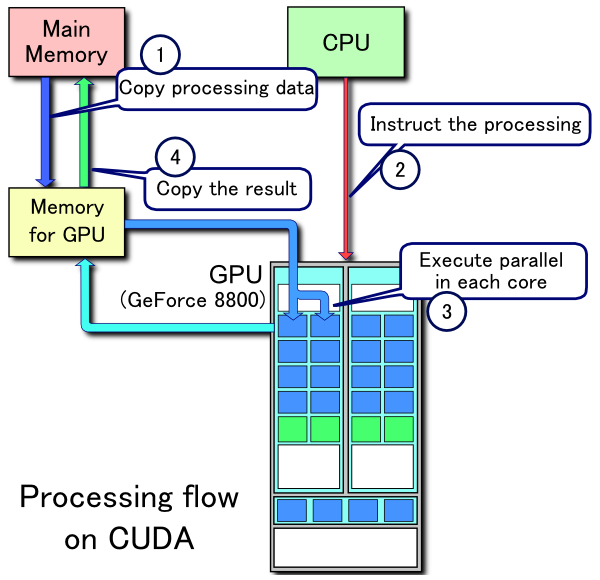
\includegraphics[width=0.3\textwidth]{images/cuda/cudaflow}
\end{figure}
1. Copy data from main memory to GPU memory.\\
2. CPU instructs the process to GPU.\\
3. GPU execute parallel in each core.\\
4. Copy the result from GPU memory to main memory.

\end{frame}


\begin{frame}{CUDA}
\begin{figure}[hH]
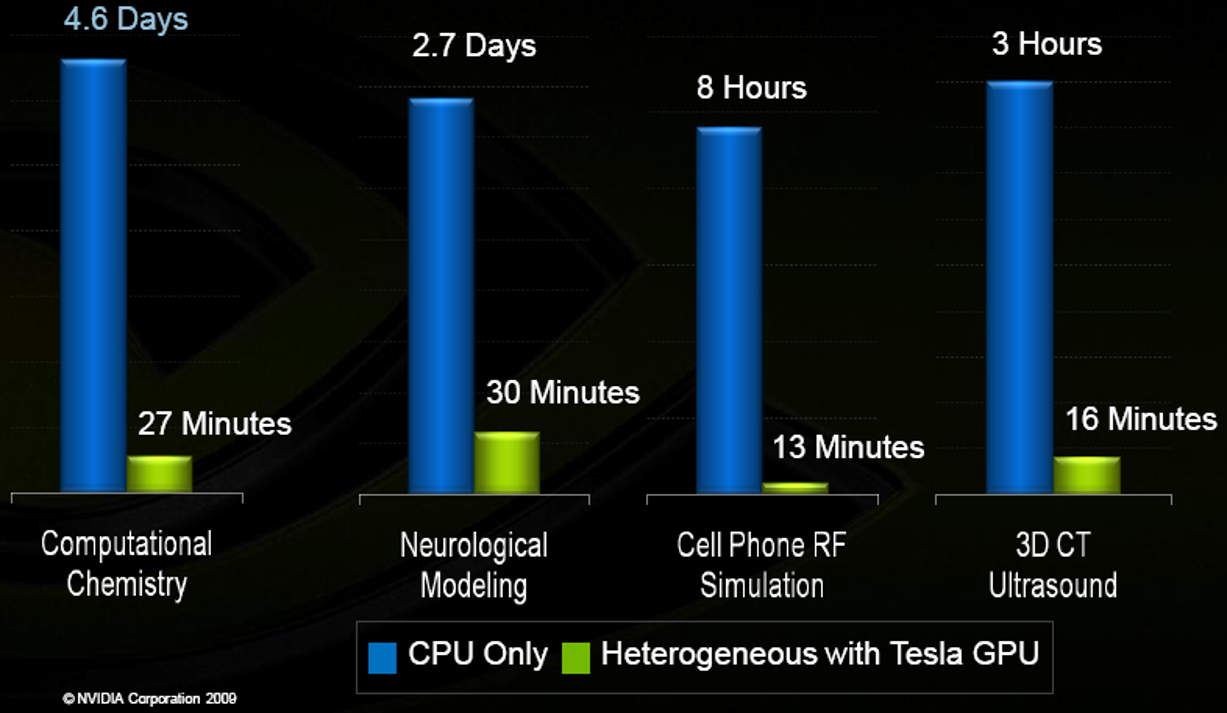
\includegraphics[width=0.5\textwidth]{images/pic1}
\end{figure}
Comparison released by Nvidia for different simulations fields.
\end{frame}

\begin{frame}
Sample C implementation for CUDA
\lstII

\end{frame}

\begin{frame}
Sample CUDA Kernel\\
\lstIII
\begin{itemize}
\item CUDA uses kernel functions. These functions are called from device (GPU) and are executed on it simultaneously by many threads in parallel.
\item There are several built in variables that are available to kernel call:\\
blockIdx - block index within grid.\\
threadIdx - thread index within block.\\
blockDim - number of threads in a block.
\end{itemize}
\end{frame}


\begin{frame}
\textbf{CUDA execution flow}
\begin{itemize}
\item At application start of execution CUDA's compiled code runs like any other application. Its primary execution is happening in CPU.
\item When kernel call is made, application continue execution of non-kernel function on CPU. In the same time, kernel function does its execution on GPU. This way we get parallel processing between CPU and GPU.  
\item Memory move between host and device is primary bottleneck in application execution. Execution on both is halted until this operation completes.
\end{itemize}
\end{frame}



\begin{frame}{Results}{}
\begin{center}
\textbf{Results}
\end{center}
\end{frame}


\begin{frame}{Results}{Steady State}
\textbf{Steady State - Lid Driven Cavity}\linebreak

The problem geometry is simple and two-dimensional. Problem domain consists of a square block filled with some incompressible fluid, where top lid is constantly moving with constant velocity in fixed direction while other three walls are solid.\linebreak

The flow pattern generated by fluid particles in this given circumstances can be simulated using Gauss-Seidel iterator on previously mentioned discritized form of Steady State Navier-Stokes (\ref{spsi}) and Continuity equation (\ref{somega}).
\end{frame}

\begin{frame}{Results}{Steady State}
\begin{figure}
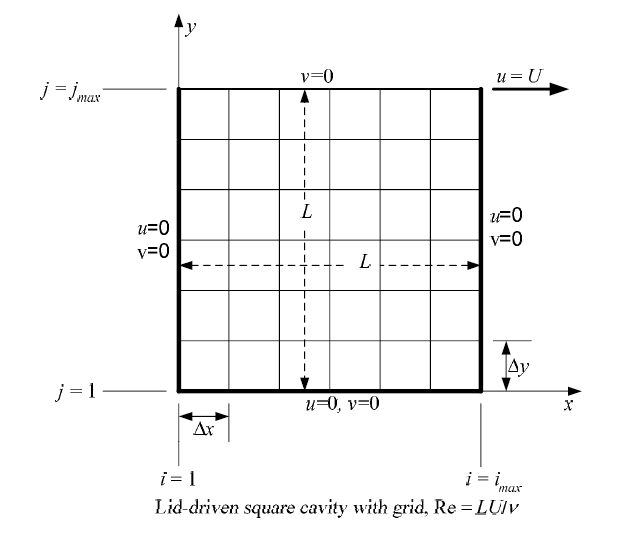
\includegraphics[width=0.8\textwidth]{images/steady/domain}
\end{figure}
\end{frame}

\begin{frame}{Results}{Steady State}

The Boundary conditions used in our problem are,
$$\psi=0, ~~~\forall i,j$$
\begin{eqnarray}
Left Wall &:& \omega_{i,j} = - \frac{2 \psi_{2,j}}{(\Delta x)^{2}} , ~~~for 2\leq j \leq j_{max-1} \nonumber\\
Right Wall &:& \omega_{imax,j} = - \frac{2 \psi_{imax-1,j}}{(\Delta x)^{2}} , ~~~for 2\leq j \leq j_{max-1} \nonumber\\
Bottom Wall &:& \omega_{i,1} = - \frac{2 \psi_{i,2}}{(\Delta y)^{2}} , ~~~for 2\leq i \leq i_{max-1} \nonumber\\
Top Wall &:& \omega_{i,jmax} = - \frac{2 \psi_{i,jmax-1} + 2\Delta y U}{(\Delta y)^{2}} , for 2\leq i \leq i_{max-1} \nonumber
\end{eqnarray}
\end{frame}

\begin{frame}{Results}{Steady State}
\begin{figure}[hH]
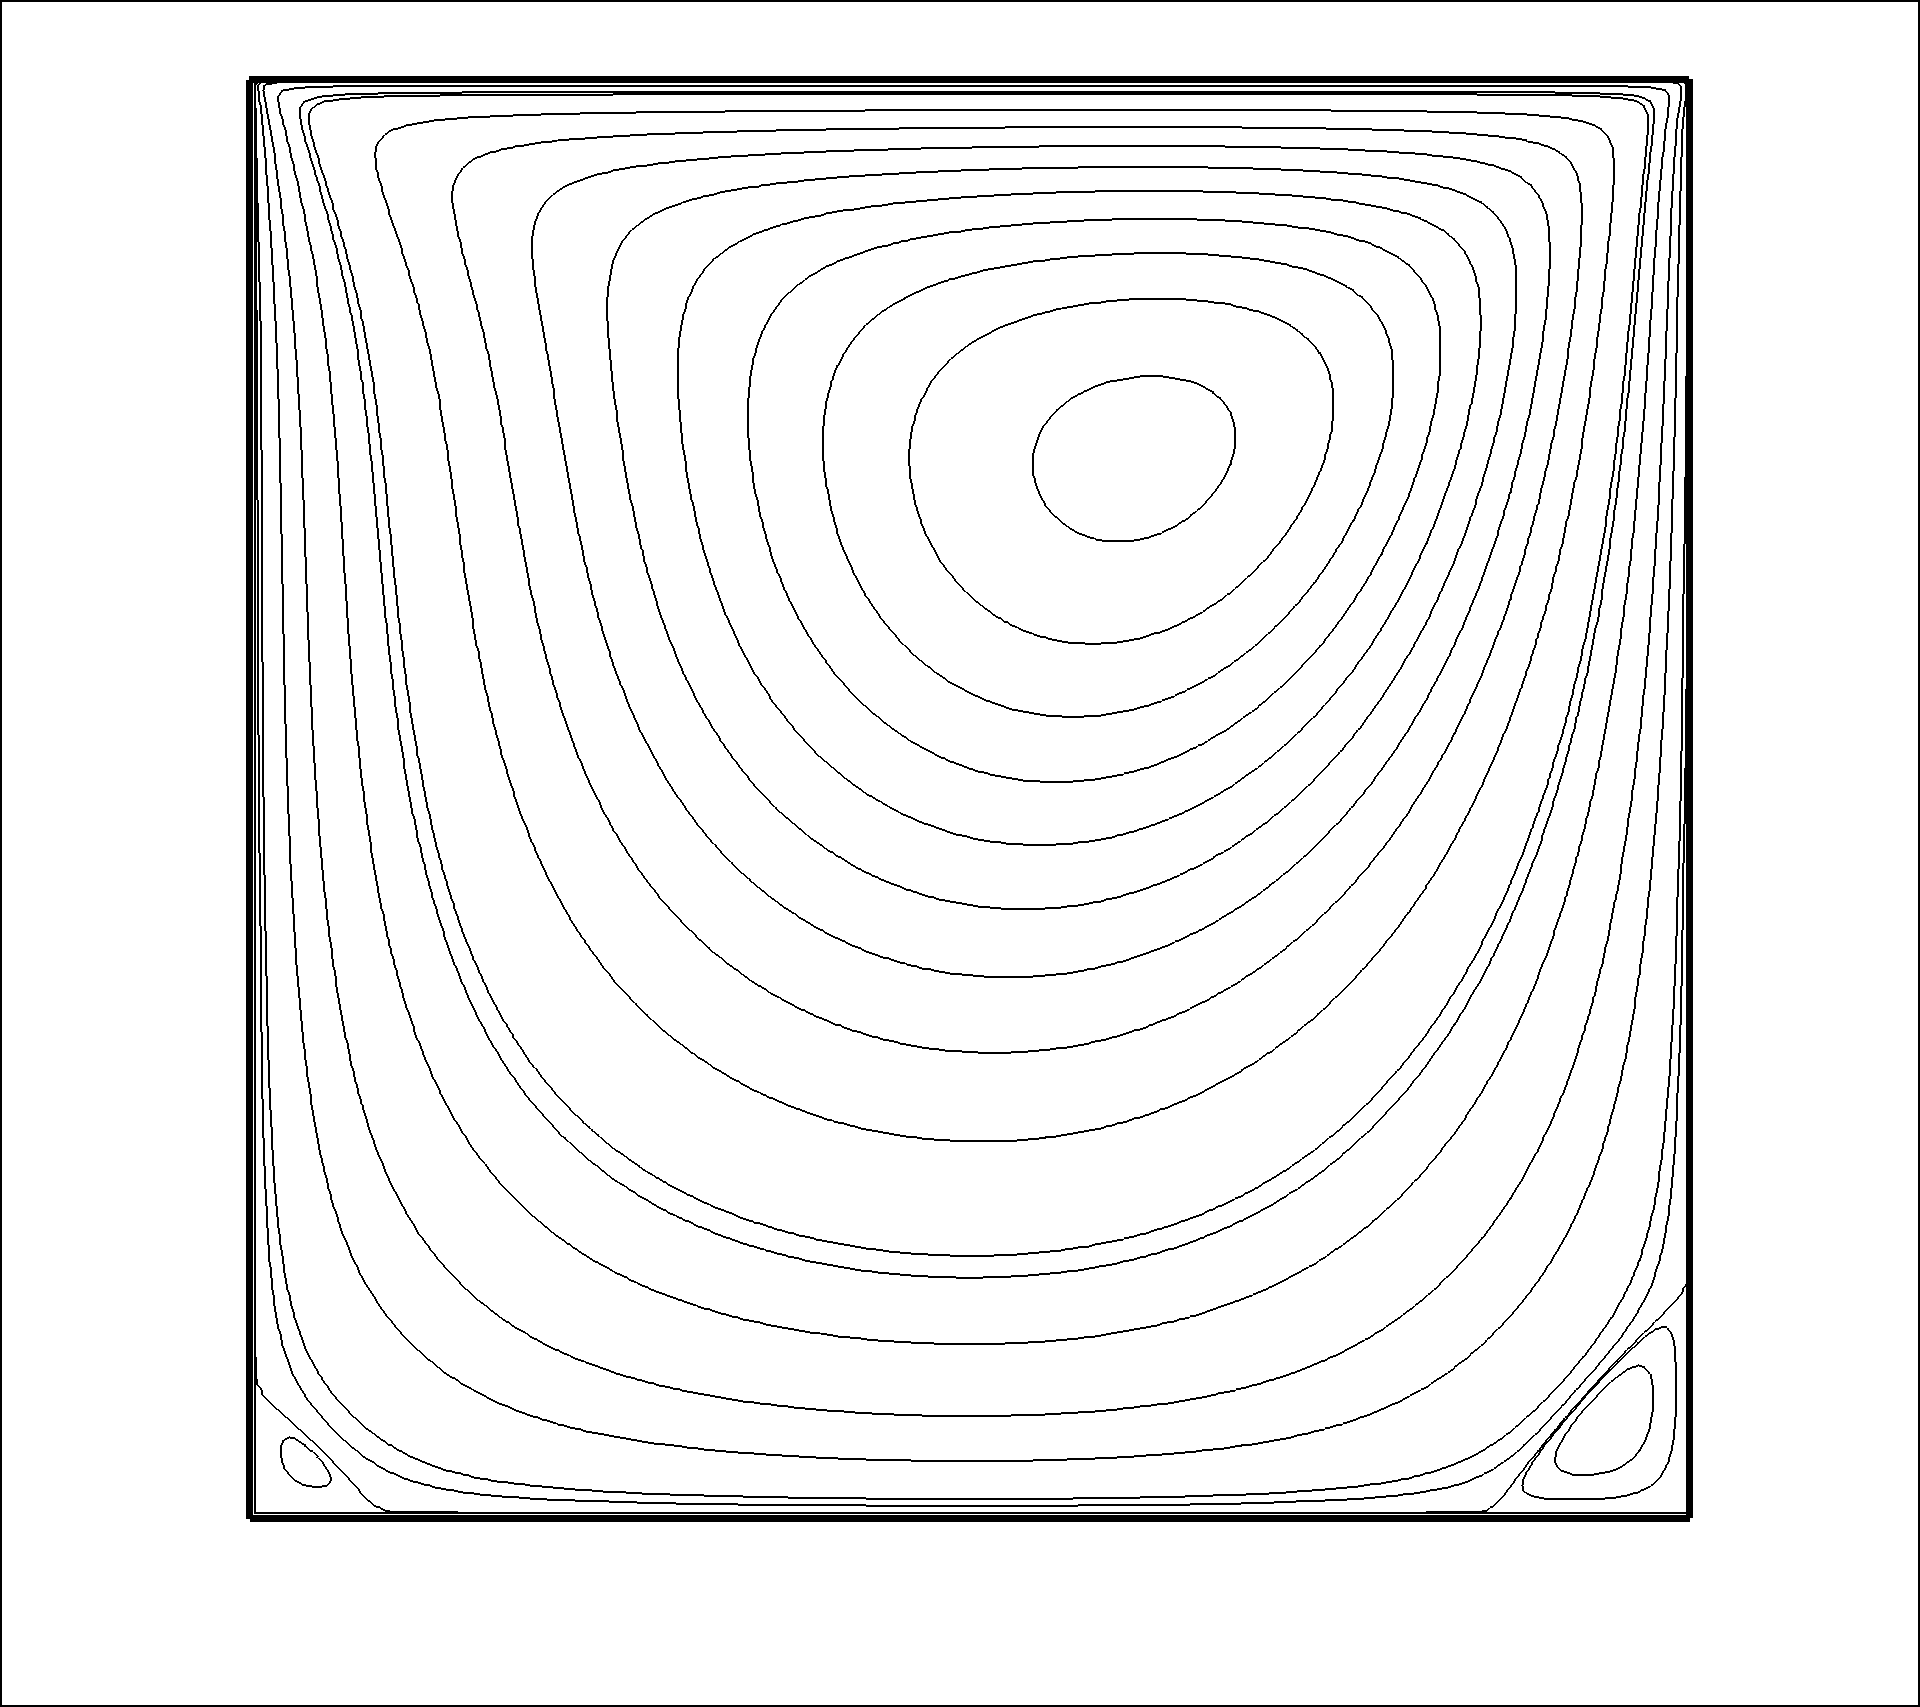
\includegraphics[width=0.25\textwidth]{images/steady/100psi}
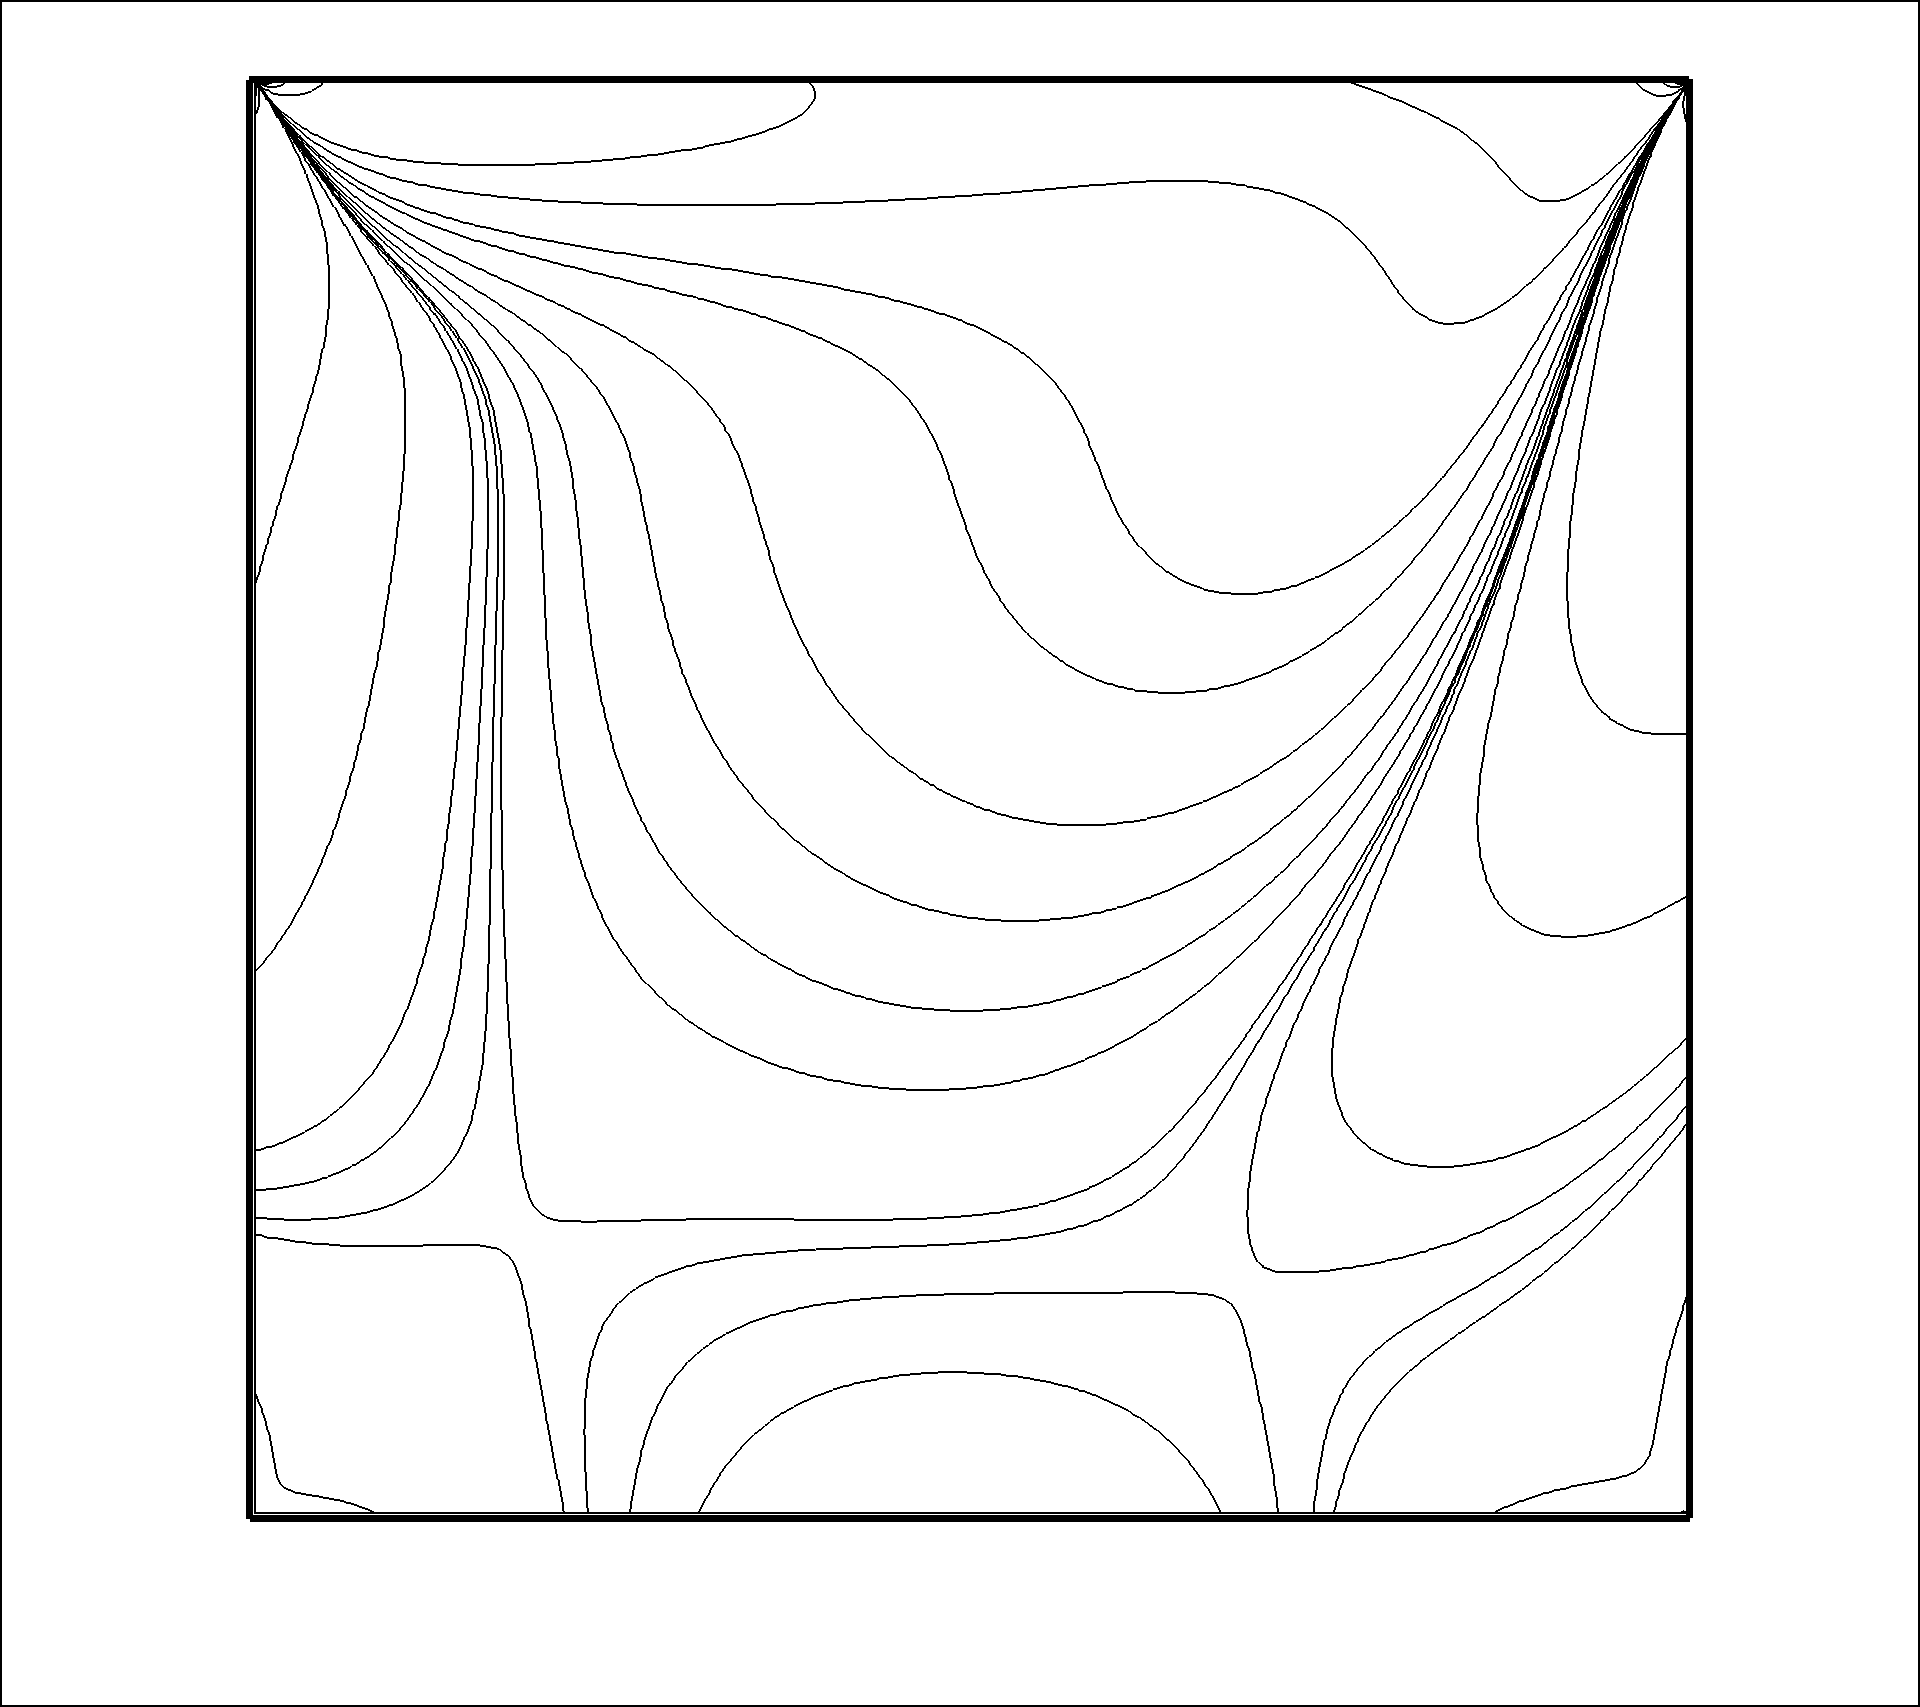
\includegraphics[width=0.25\textwidth]{images/steady/100omega}\\
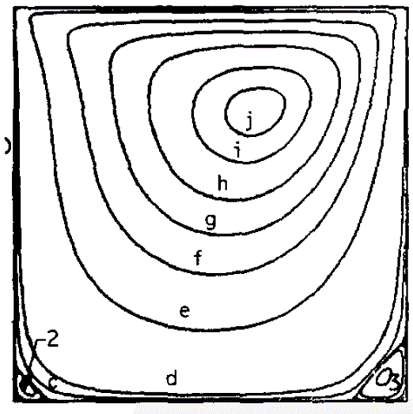
\includegraphics[width=0.25\textwidth]{images/steady/ghia100psi}
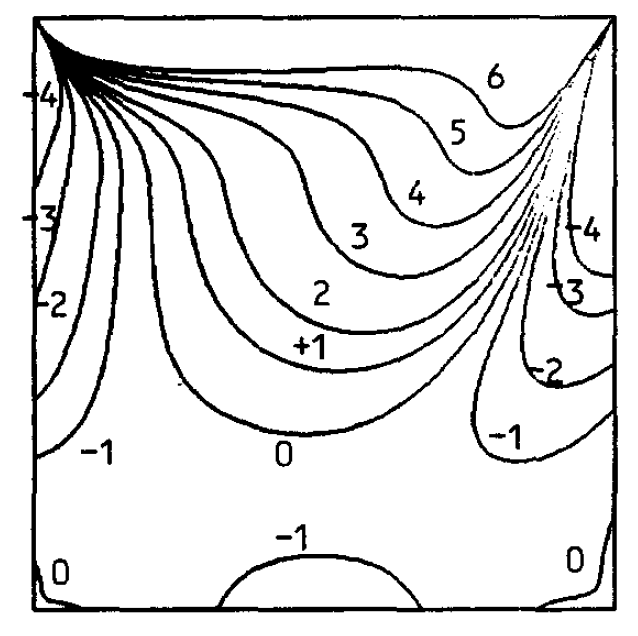
\includegraphics[width=0.25\textwidth]{images/steady/ghia100omega}
\caption{Streamlines and Vorticity Plot. Our Results vs Ghia, et al [1] at Re 100}
\end{figure}
\end{frame}

\begin{frame}{Results}{Steady State}
\begin{figure}
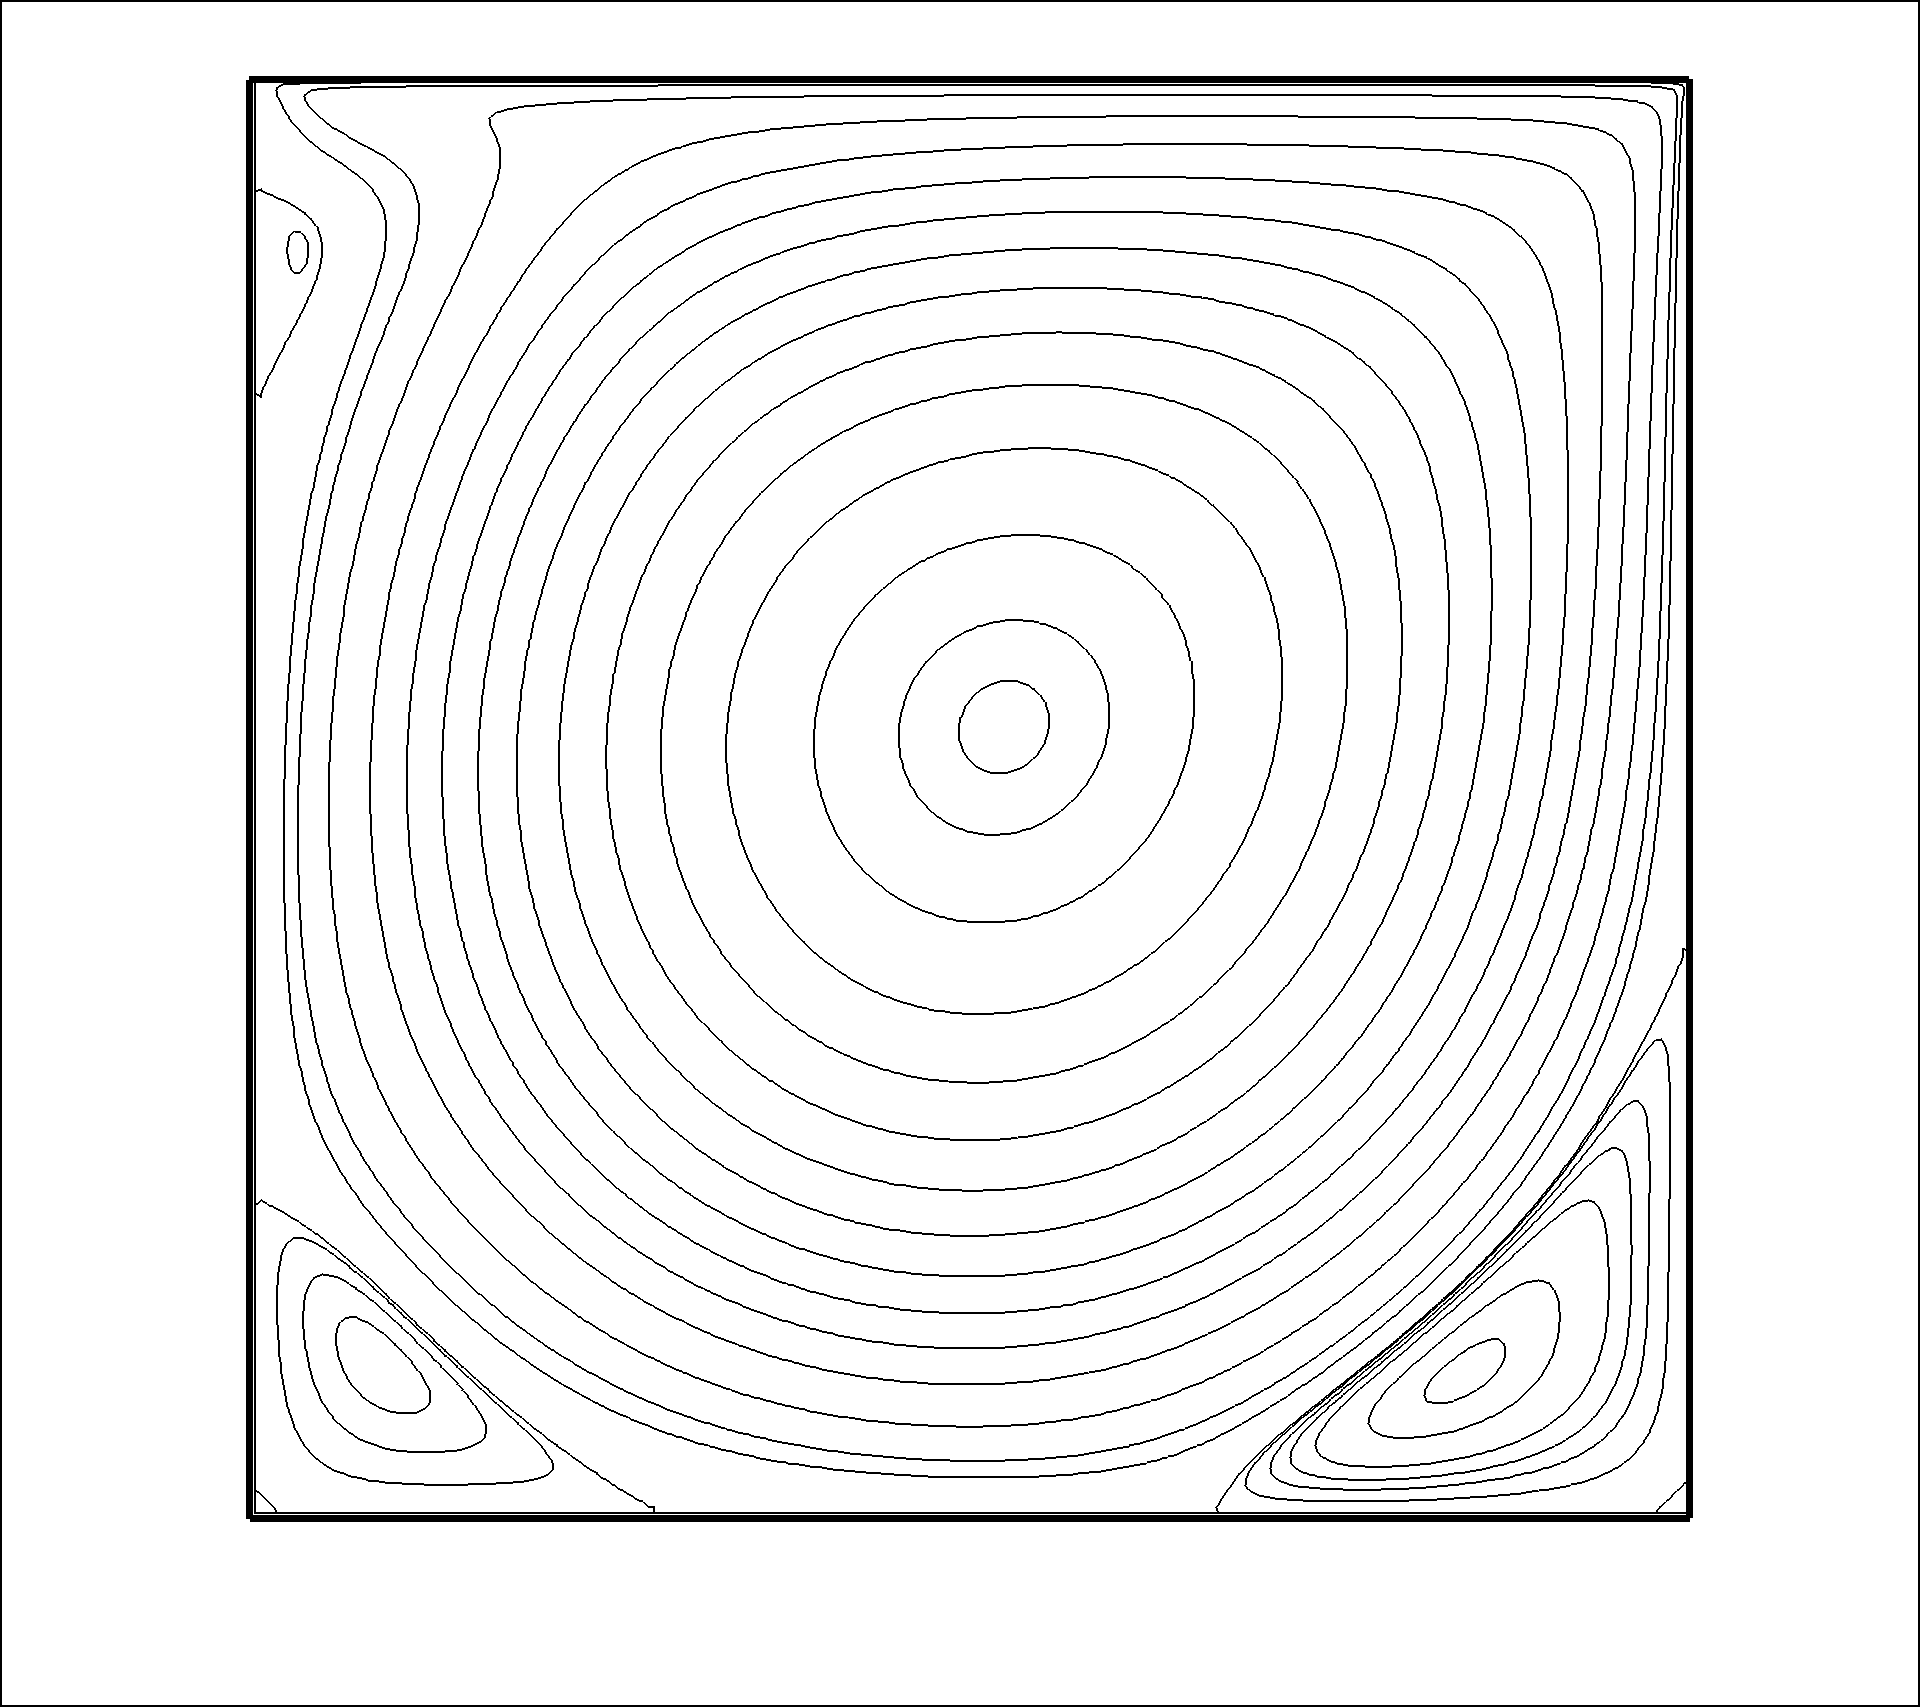
\includegraphics[width=0.49\textwidth]{images/steady/2000psi}
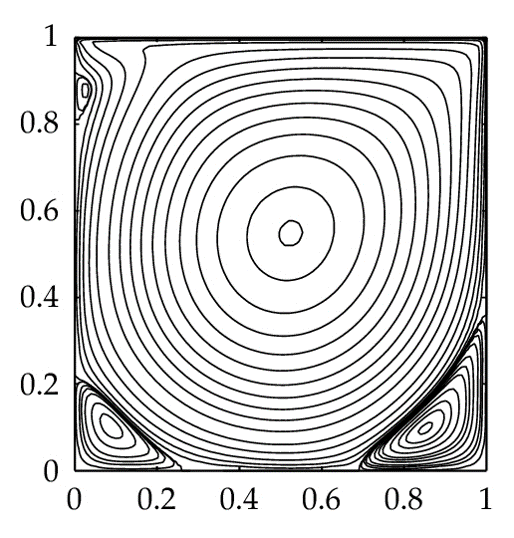
\includegraphics[width=0.49\textwidth]{images/steady/k2000psi}
\caption{Streamlines Plot. Our Results vs K. Poochinapan [2] at Re 2000}
\end{figure}
\end{frame}


\begin{frame}{Results}{Unsteady State}
\textbf{Unsteady State}\linebreak

The problem is to find the evolution of flow of a incompressible viscous fluid in a square domain where the top lid is moving with velocity U. The problem domain and boundary conditions are same as Steady State.
\begin{figure}
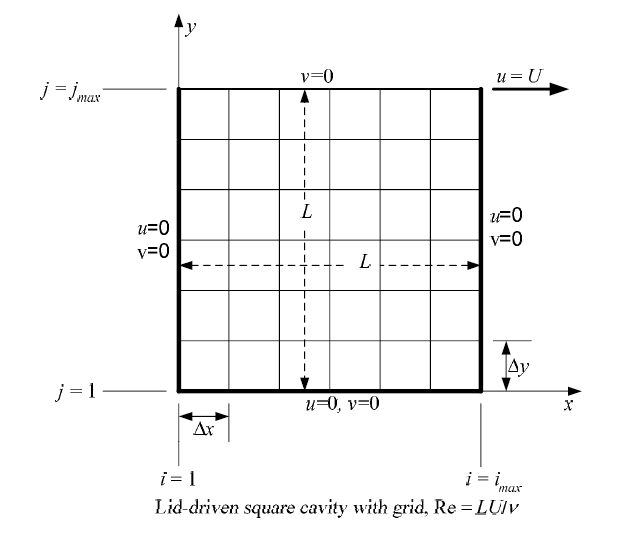
\includegraphics[width=0.5\textwidth]{images/steady/domain}
\end{figure}
\end{frame}

\begin{frame}{Results}{Unsteady State}
\begin{figure}[hH]
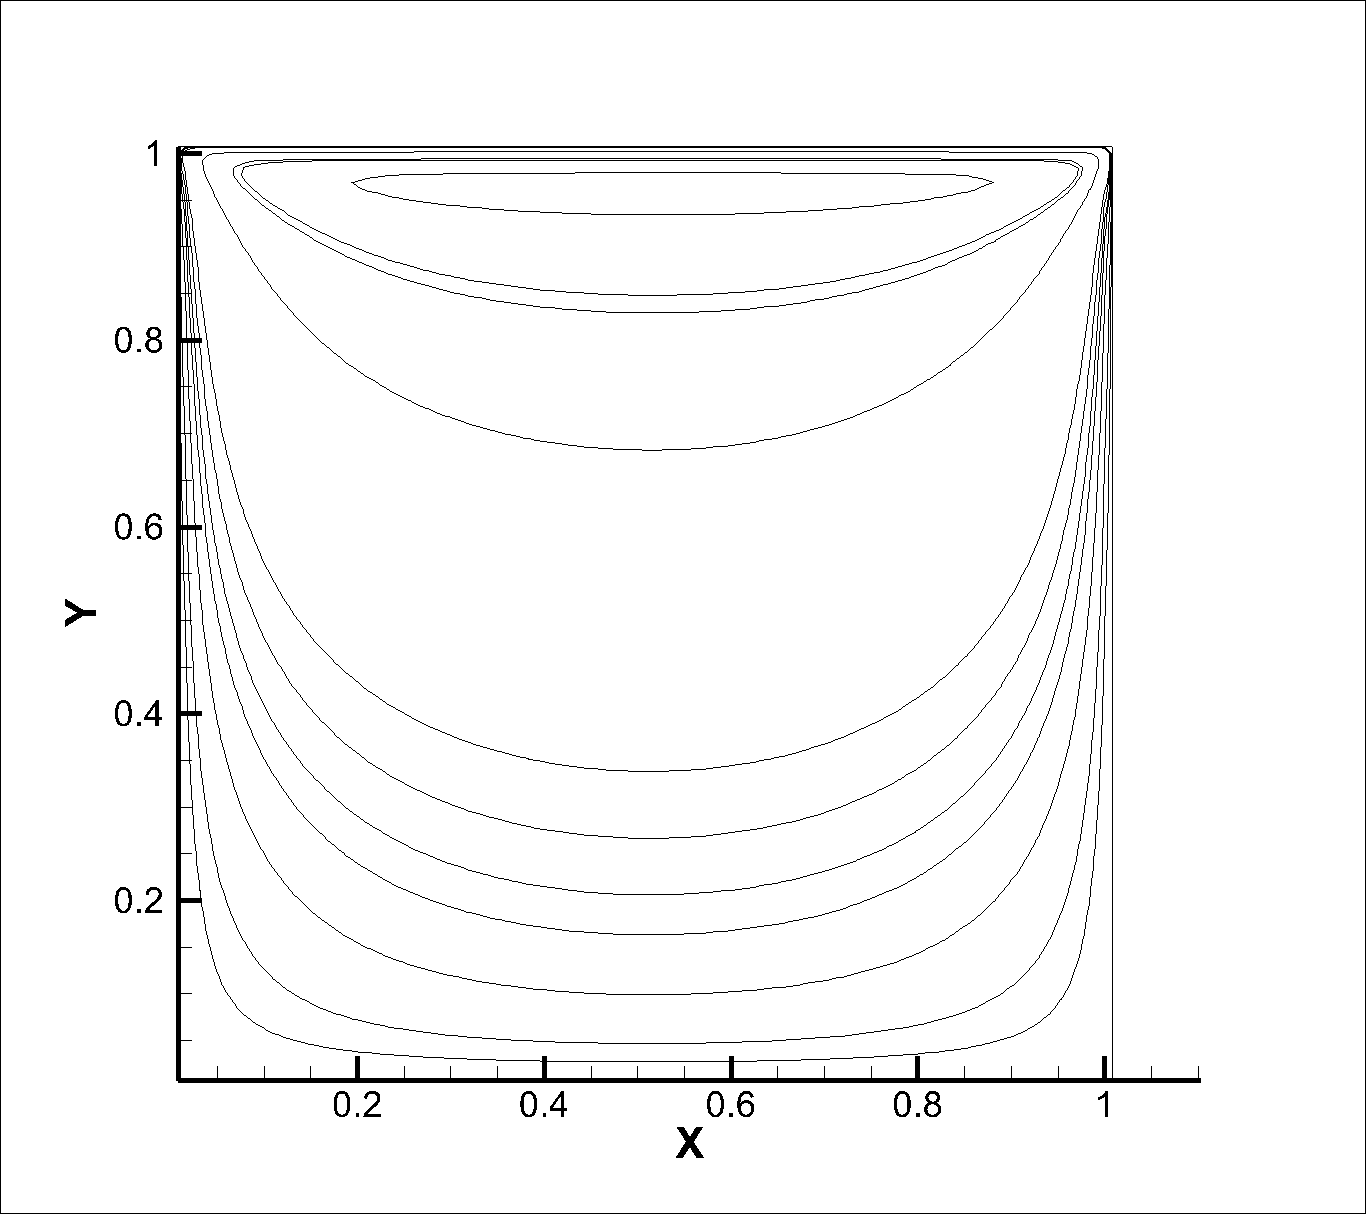
\includegraphics[width=0.25\textwidth]{images/unsteady/re40010}
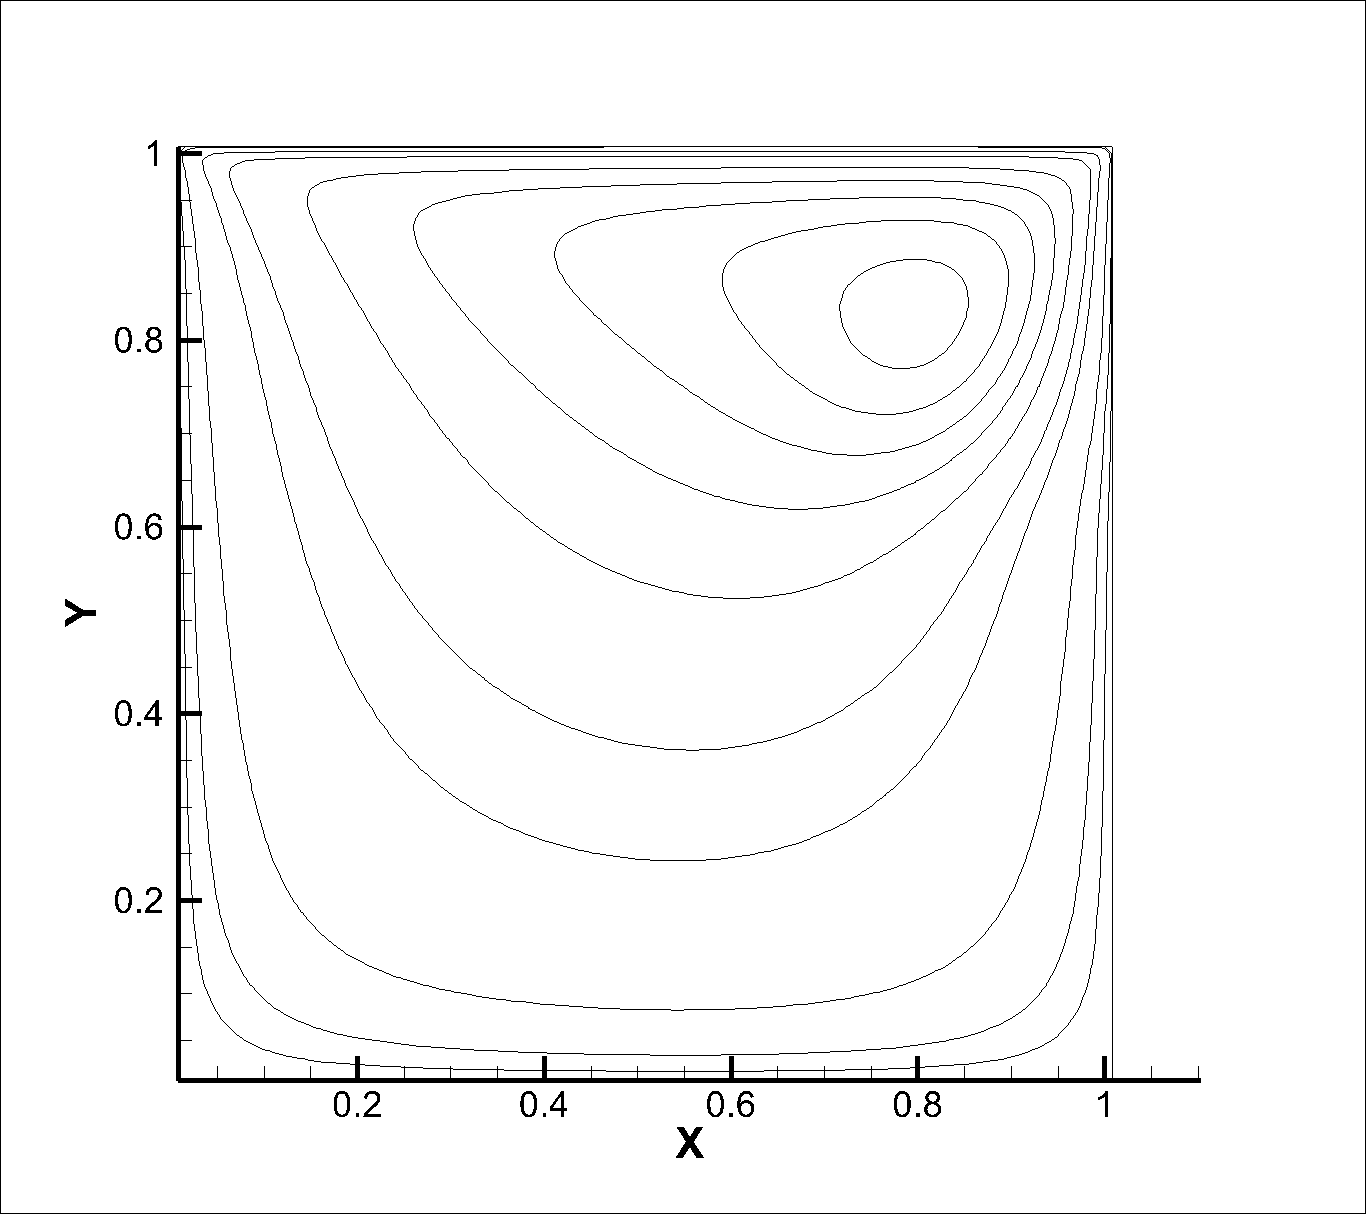
\includegraphics[width=0.25\textwidth]{images/unsteady/re40011}
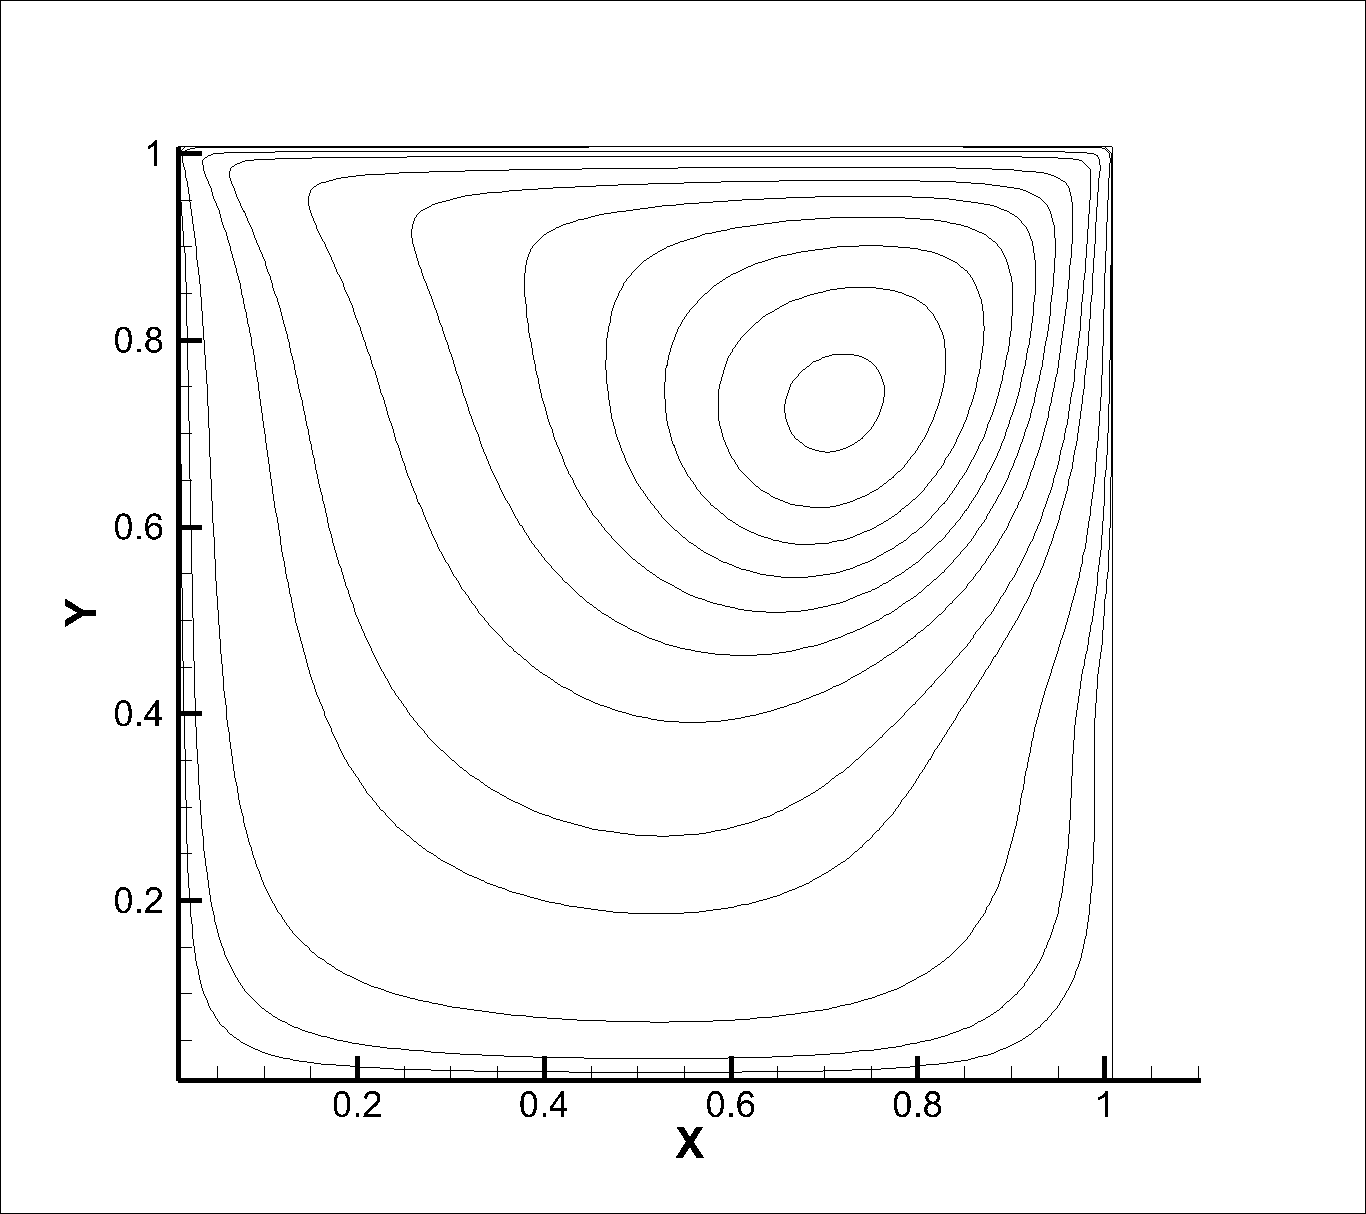
\includegraphics[width=0.25\textwidth]{images/unsteady/re40012}
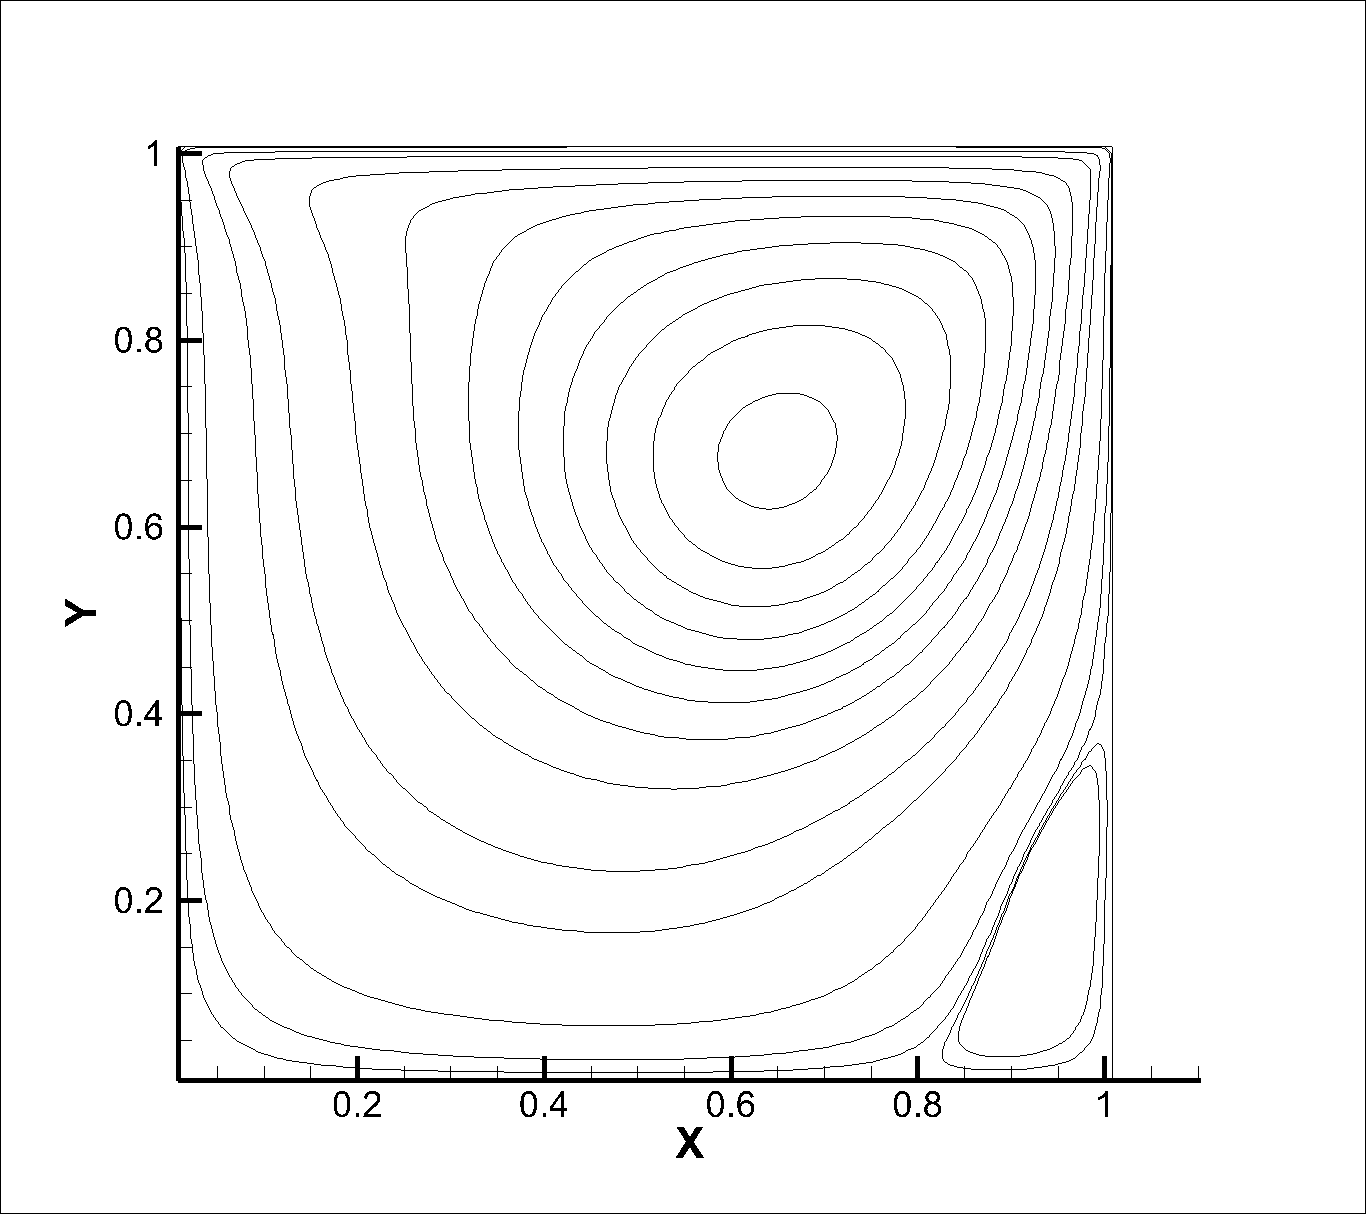
\includegraphics[width=0.25\textwidth]{images/unsteady/re40013}\linebreak
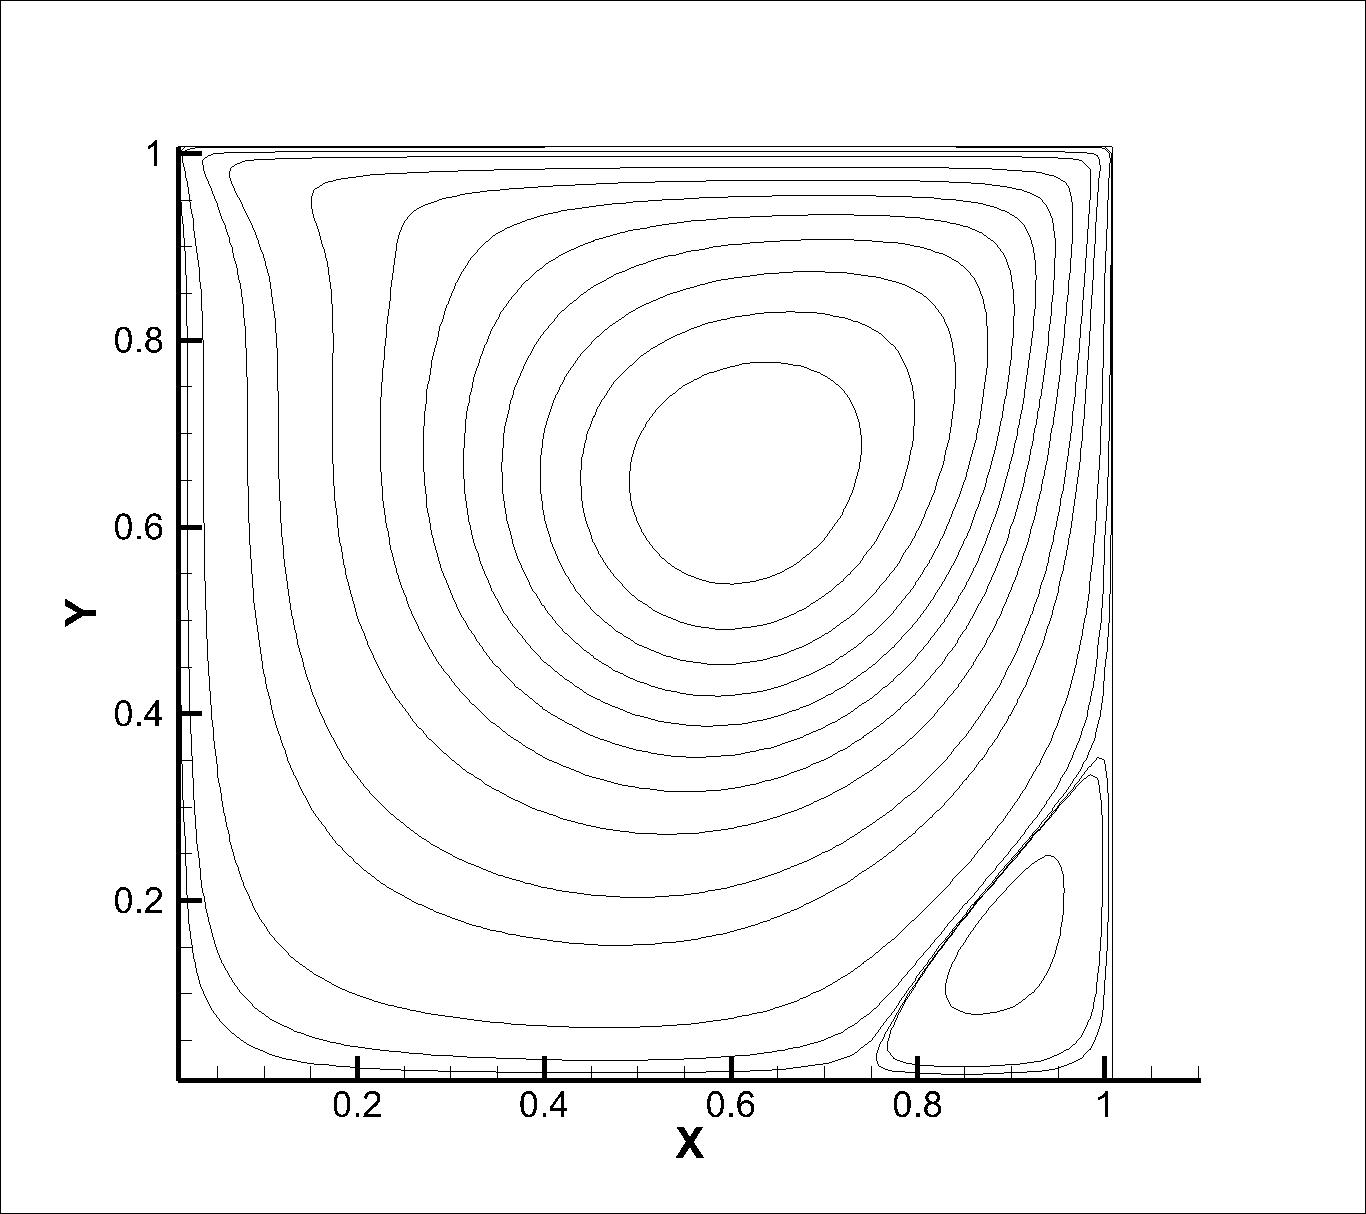
\includegraphics[width=0.25\textwidth]{images/unsteady/re4001}
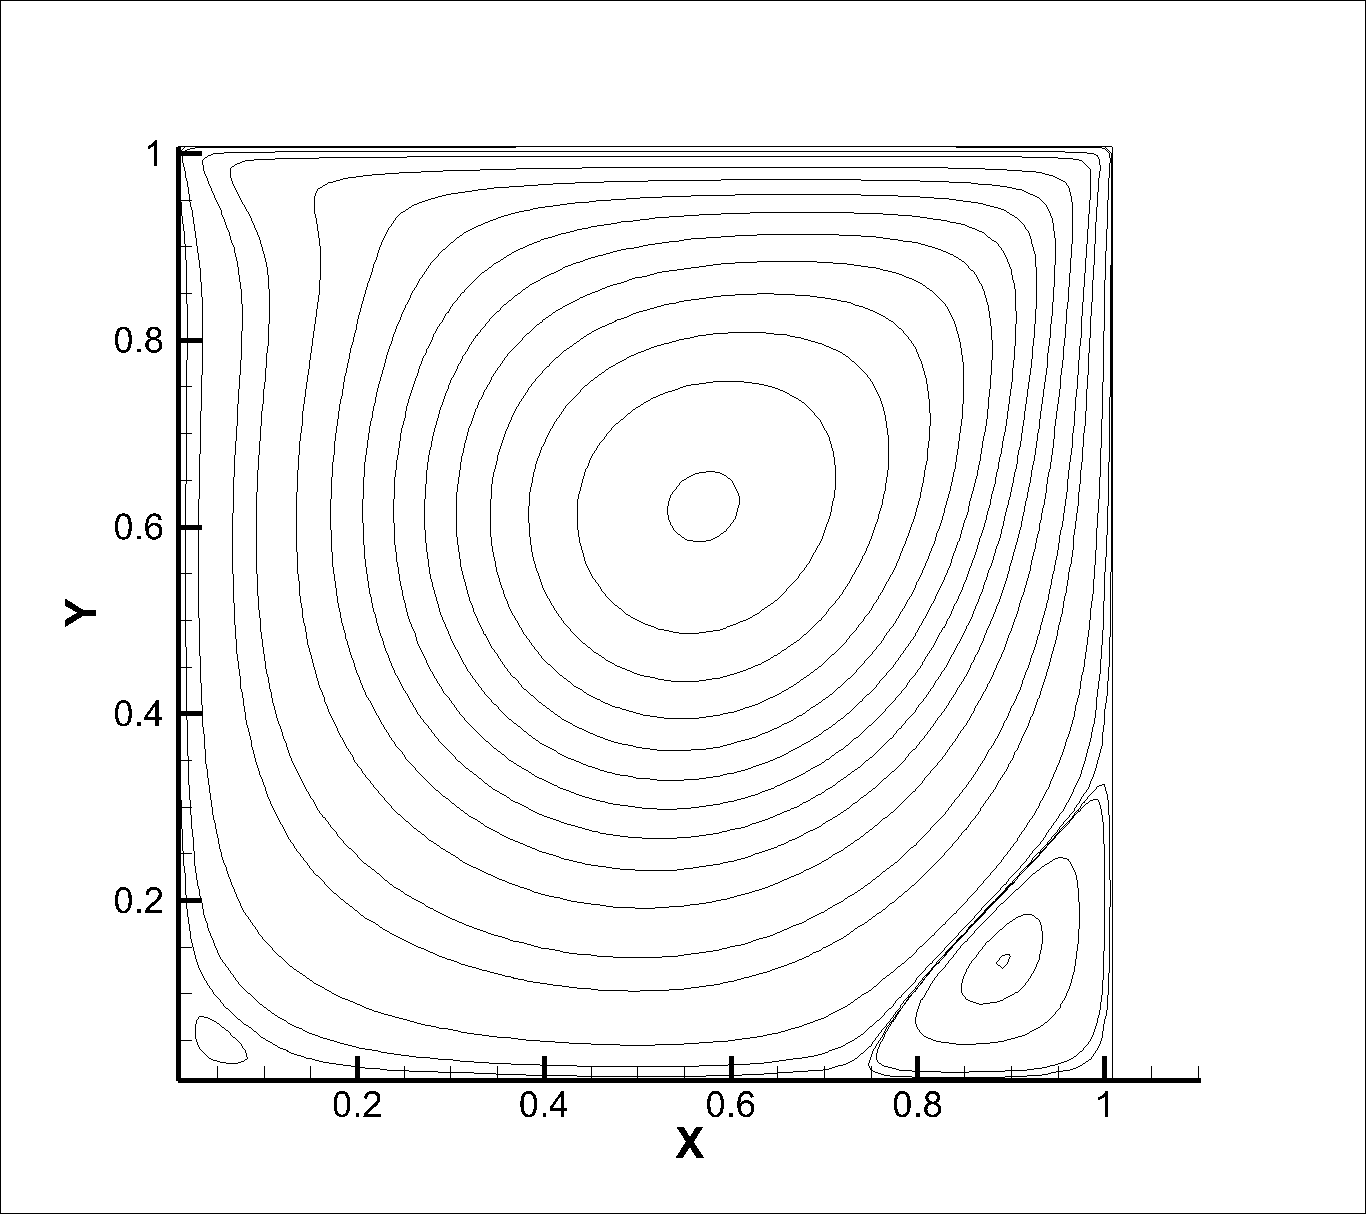
\includegraphics[width=0.25\textwidth]{images/unsteady/re4002}
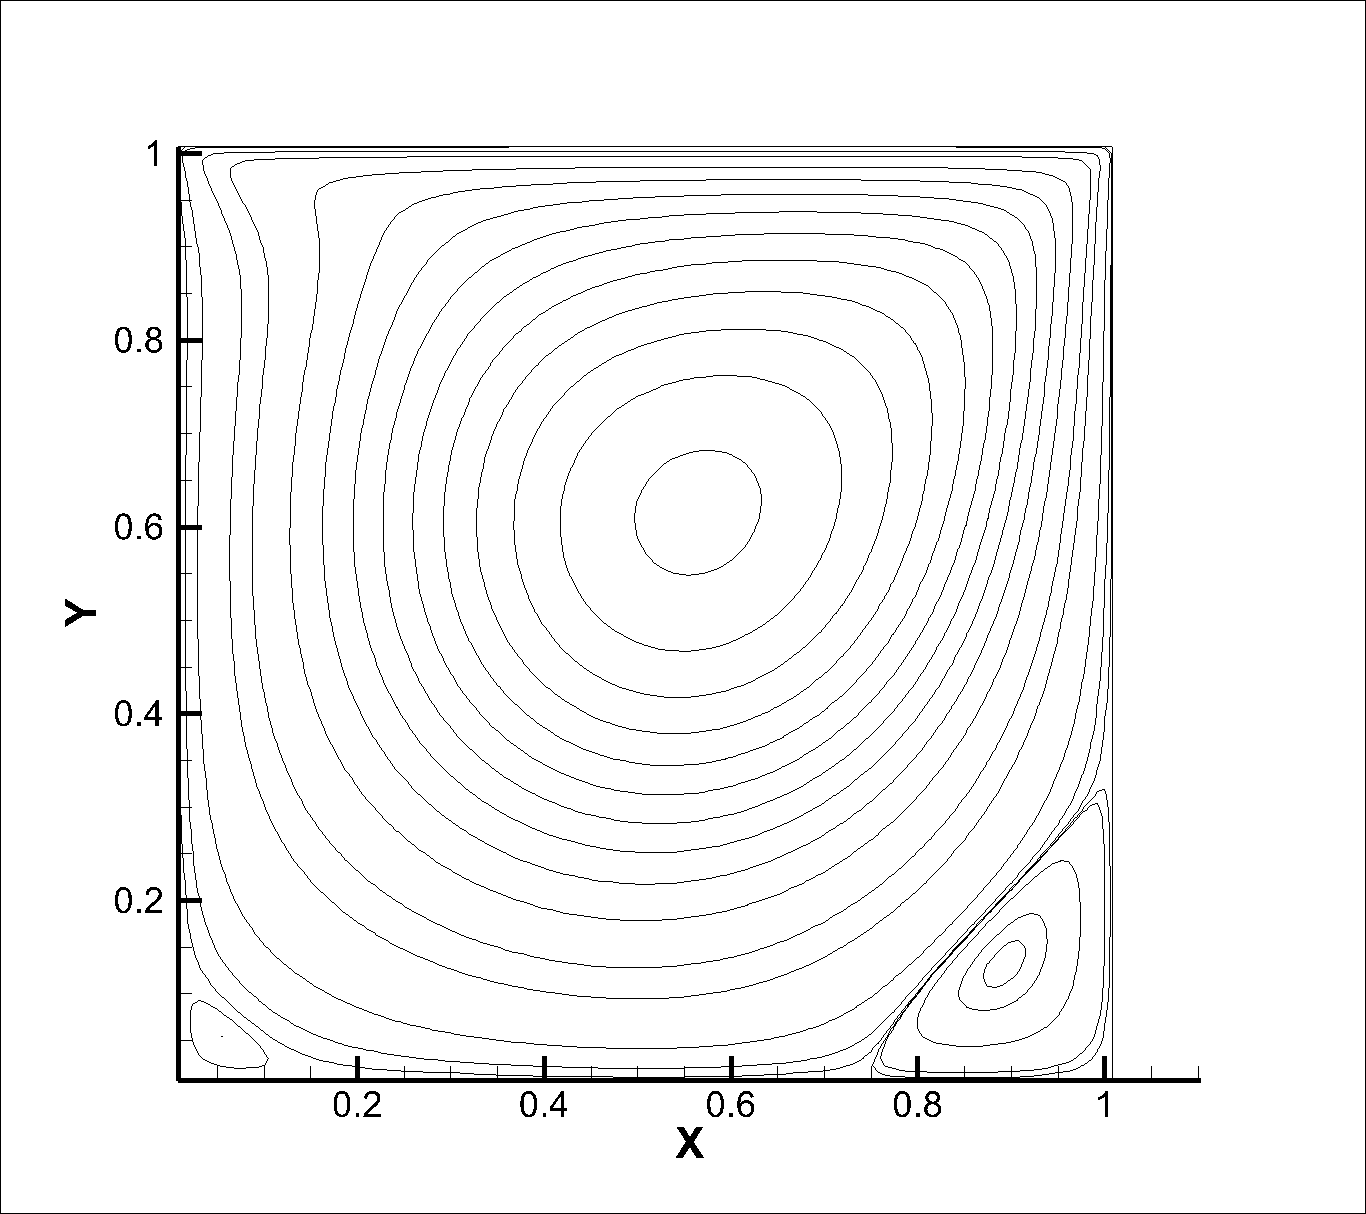
\includegraphics[width=0.25\textwidth]{images/unsteady/re4003}
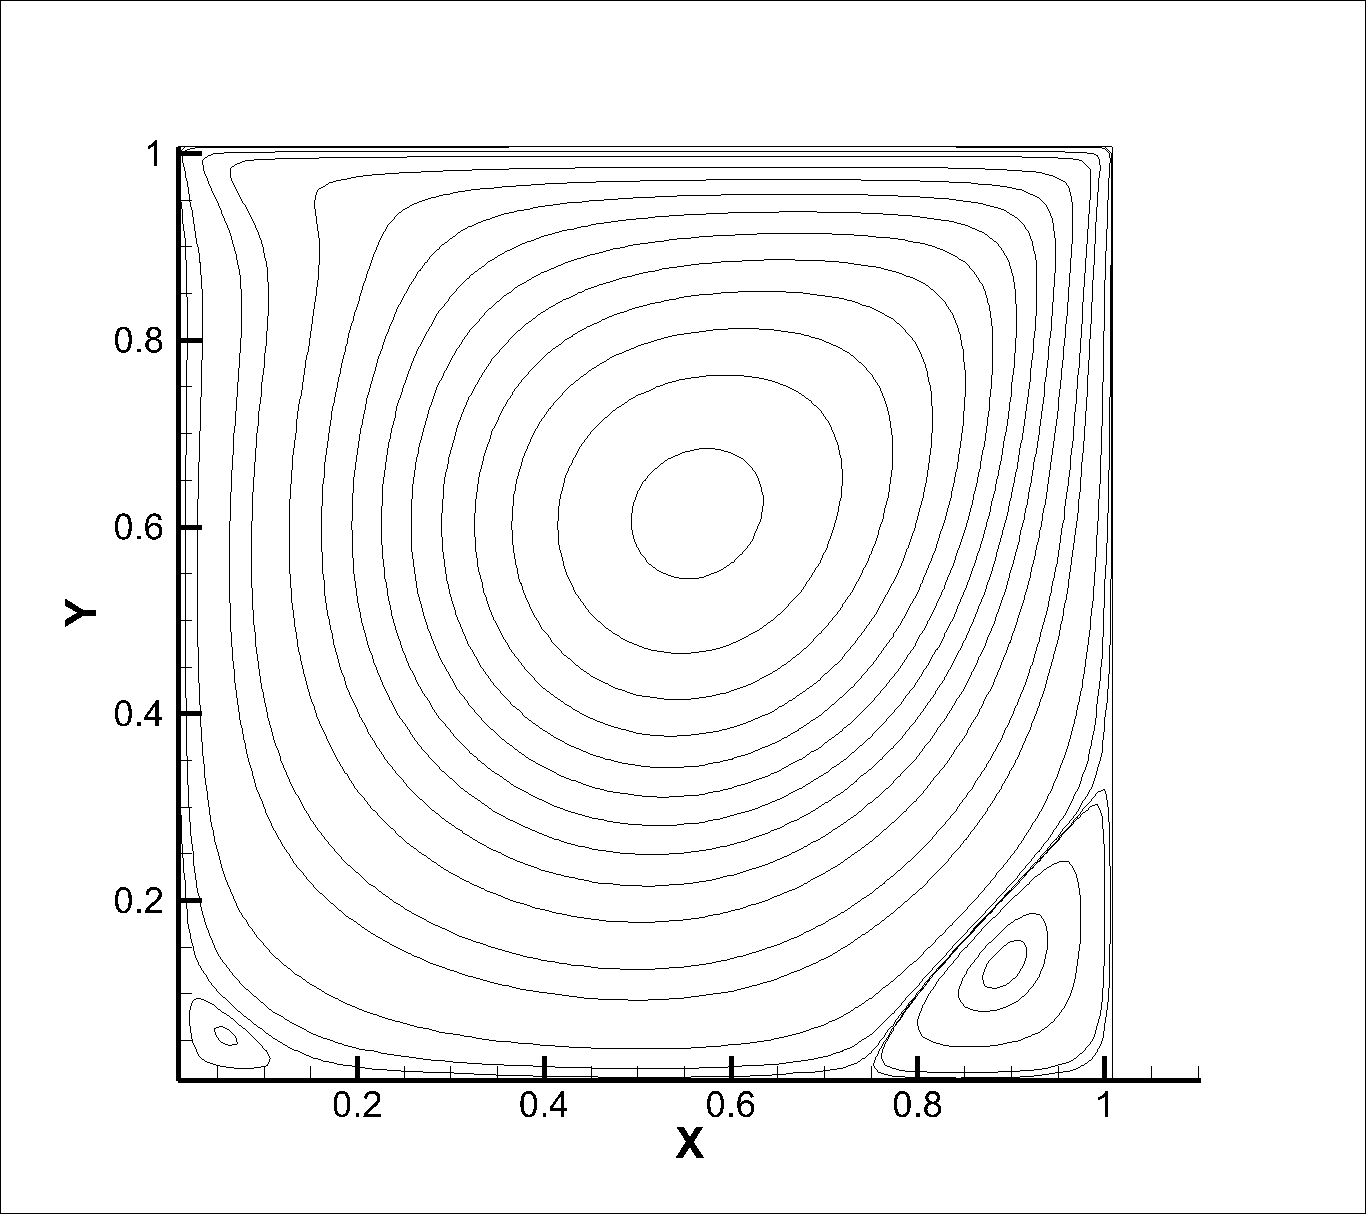
\includegraphics[width=0.25\textwidth]{images/unsteady/re4004}
\caption{The evolution of stream function in unsteady state Lid-Driven cavity for Reynolds number 400. }
\end{figure}
\end{frame}


\begin{frame}{Results}{Staggered Cavity}
\textbf{Staggered Cavity}\linebreak

The boundary conditions are same as Steady State's.
\begin{figure}[H]
\centerline{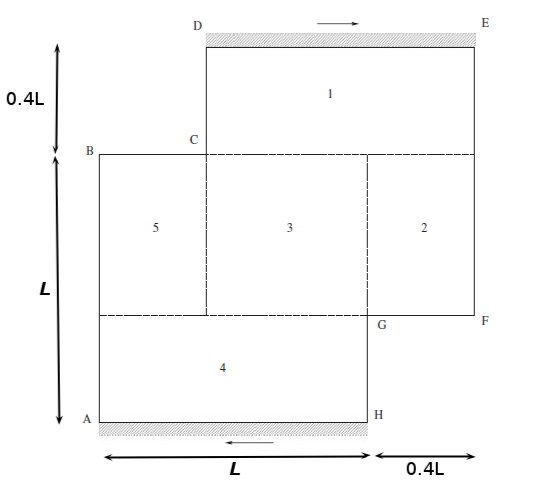
\includegraphics[width=0.4\textwidth]{images/stagerred/domain1.png}}
\caption{The problem domain for staggered cavity.}
\end{figure}
\end{frame}

\begin{frame}{Results}{Staggered Cavity}
This problem is difficult to solve because of the blocked domains at the upper left and lower right corner. To overcome this problem we had three options.
\begin{itemize}
\item  Force zero entries in the omega and psi at block domains after every iteration.
\item  Divide the domain into two smaller sub-domains and solve these domains individually.
\item  Divide the domain into five smaller sub-domains and solve these domains individually.
\end{itemize}
\begin{figure}[H]
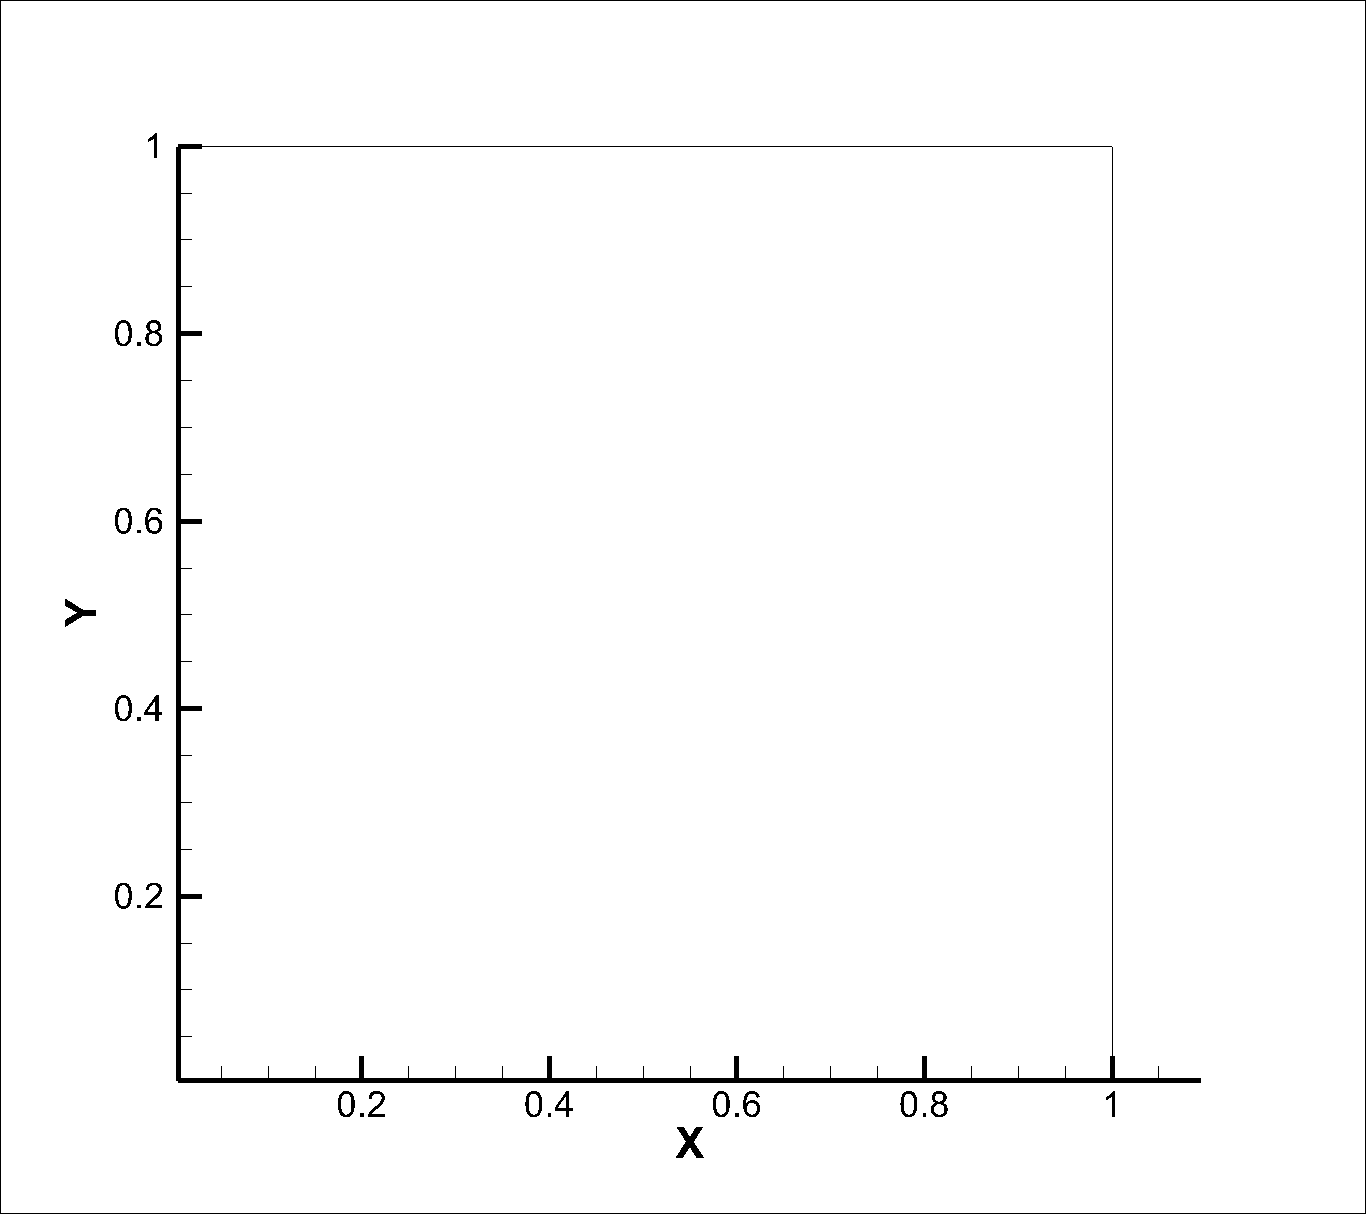
\includegraphics[width=0.25\textwidth]{images/stagerred/one}
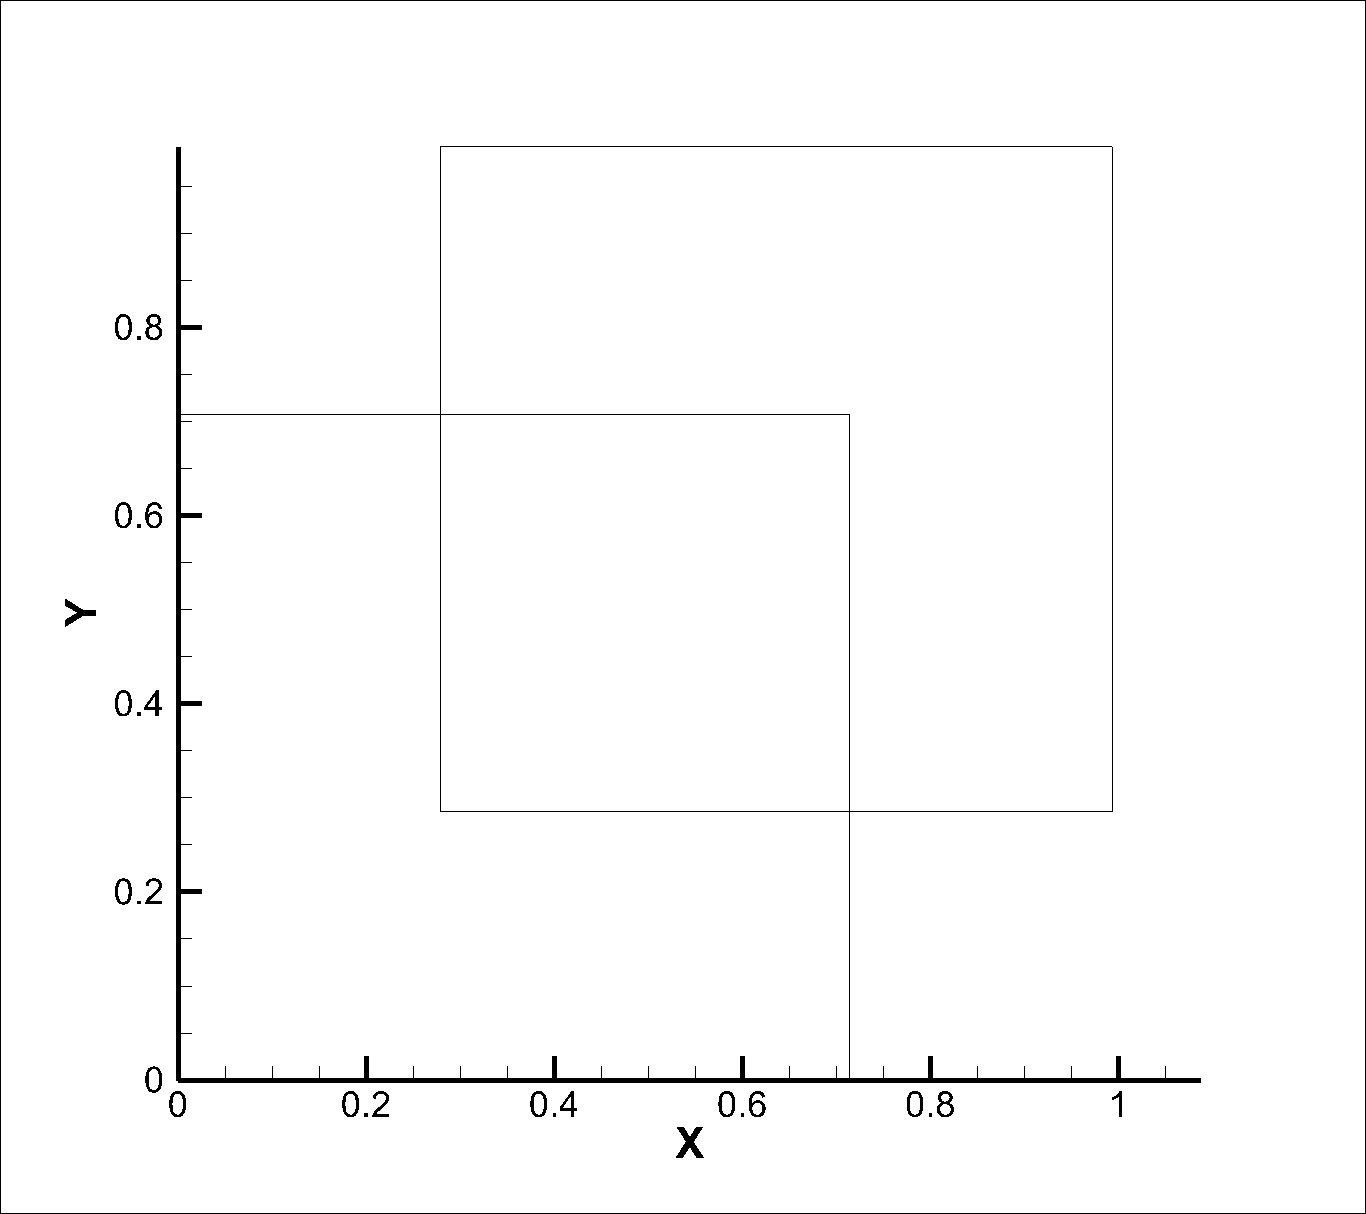
\includegraphics[width=0.25\textwidth]{images/stagerred/two}
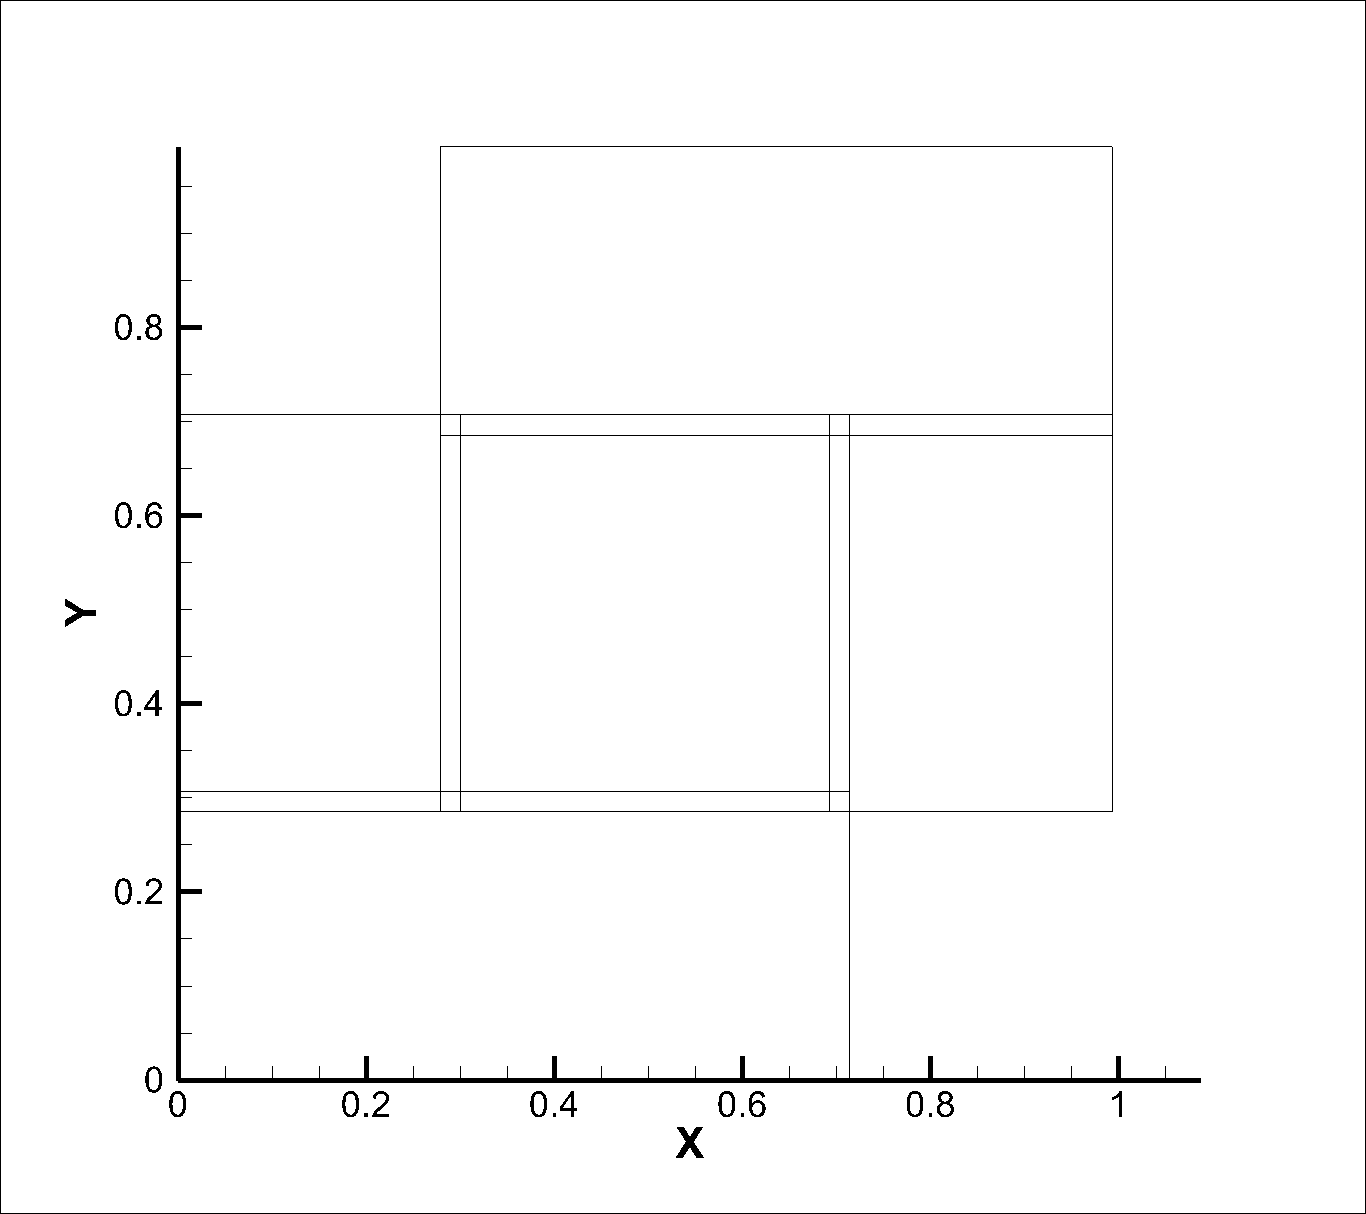
\includegraphics[width=0.25\textwidth]{images/stagerred/three}
\end{figure}
\end{frame}

\begin{frame}{Results}{Staggered Cavity}
Pseudo-Code for solving Staggered Cavity,\\
\lstI
\end{frame}

\begin{frame}{Results}{Staggered Cavity}
\begin{figure}[Hh]
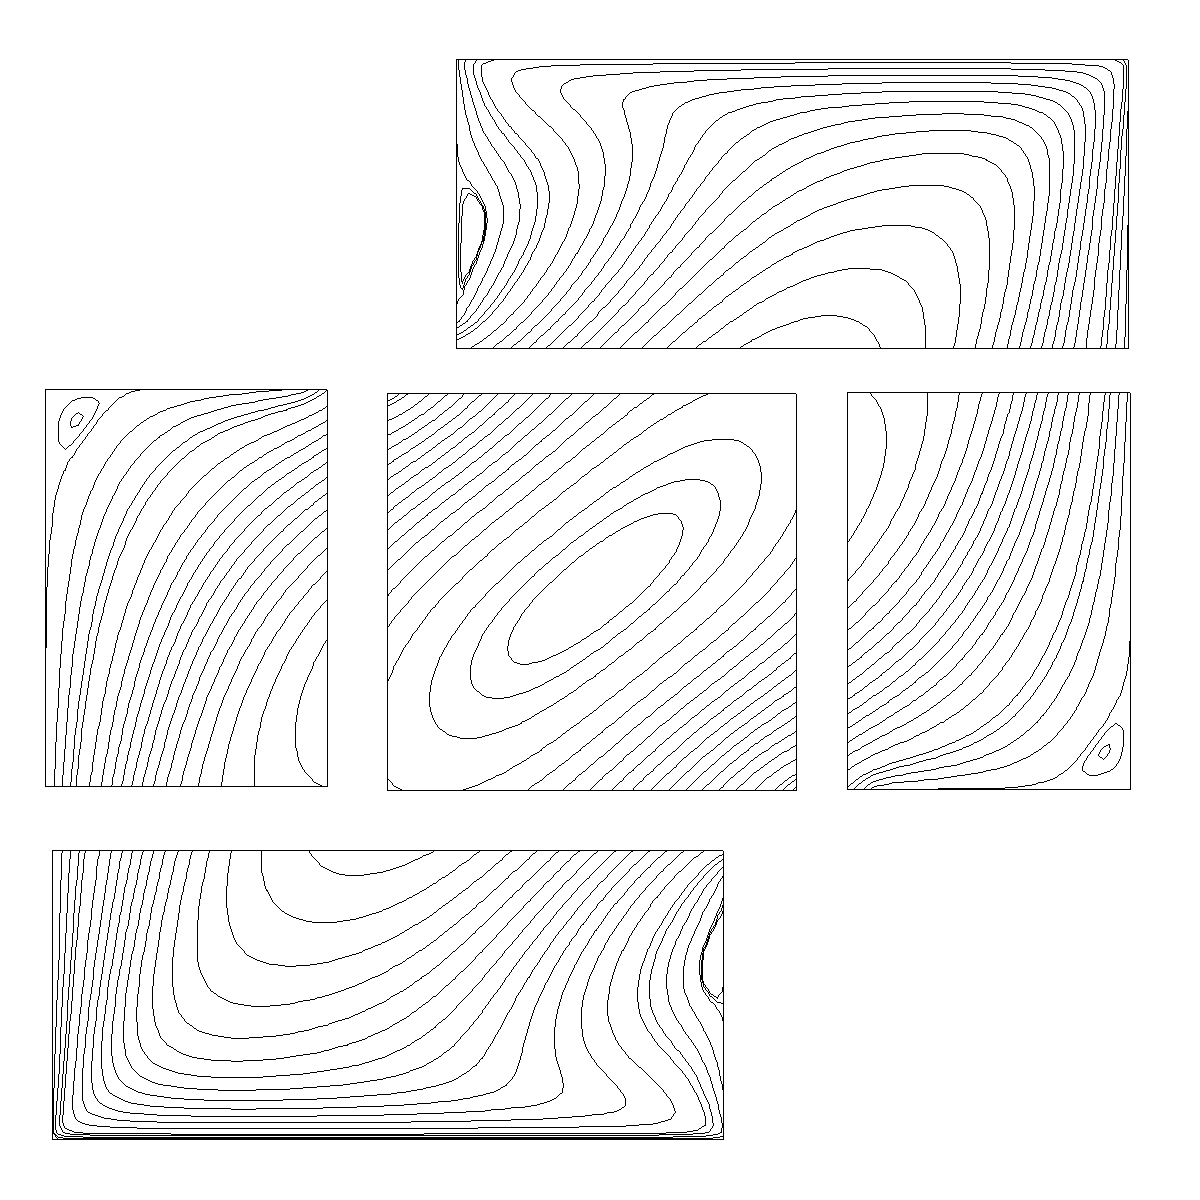
\includegraphics[width=0.49\textwidth]{images/stagerred/400block}
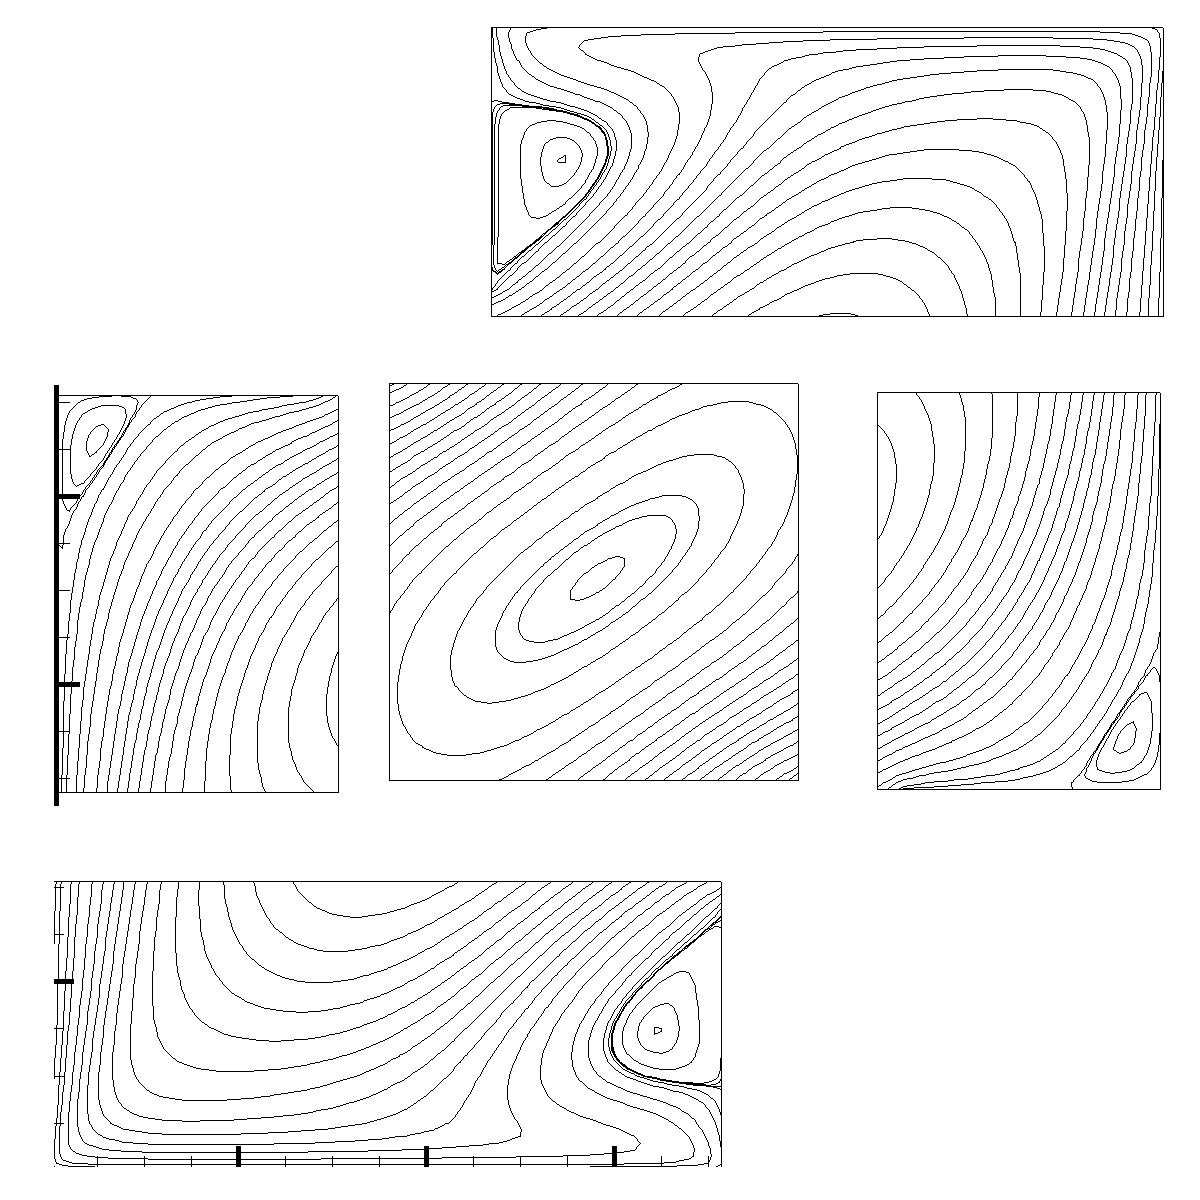
\includegraphics[width=0.49\textwidth]{images/stagerred/800block}
\caption{Streamlines calculated by diving domains into 5 subdomains at Re 400 and Re 800}
\end{figure}
\end{frame}

\begin{frame}{Results}{Staggered Cavity}
\begin{figure}
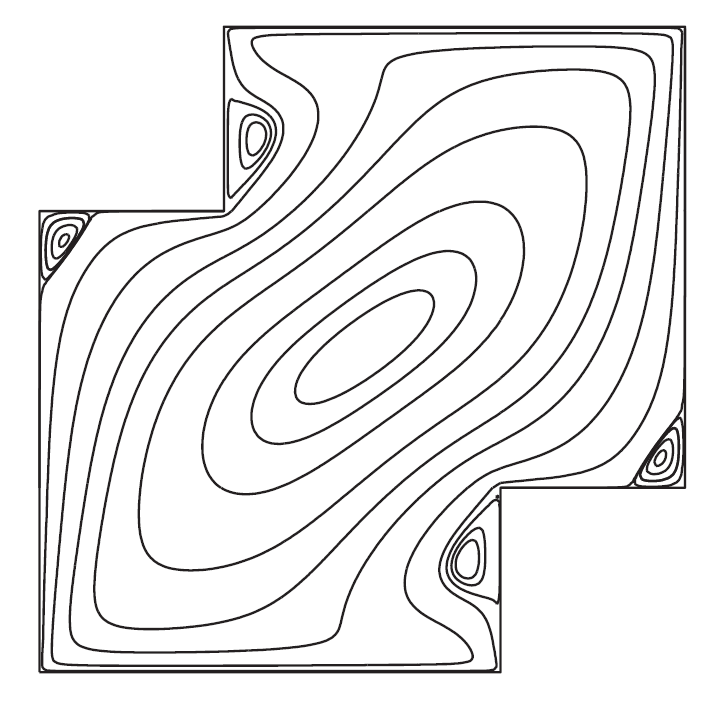
\includegraphics[width=0.25\textwidth]{images/stagerred/re400psiP}
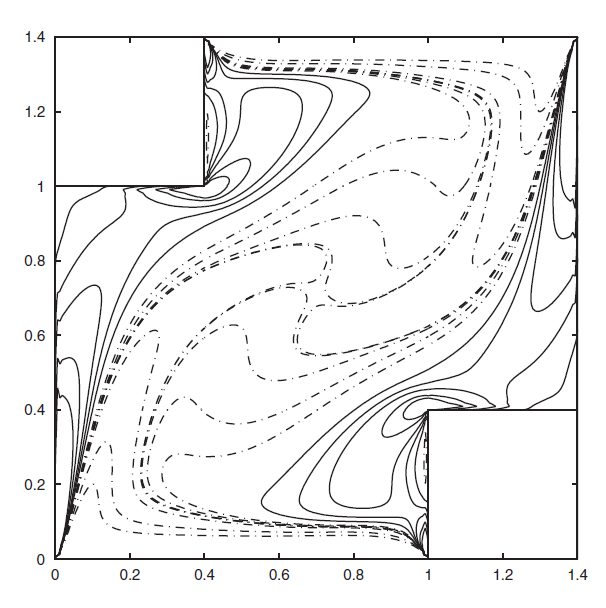
\includegraphics[width=0.25\textwidth]{images/stagerred/re400omegaP}\\
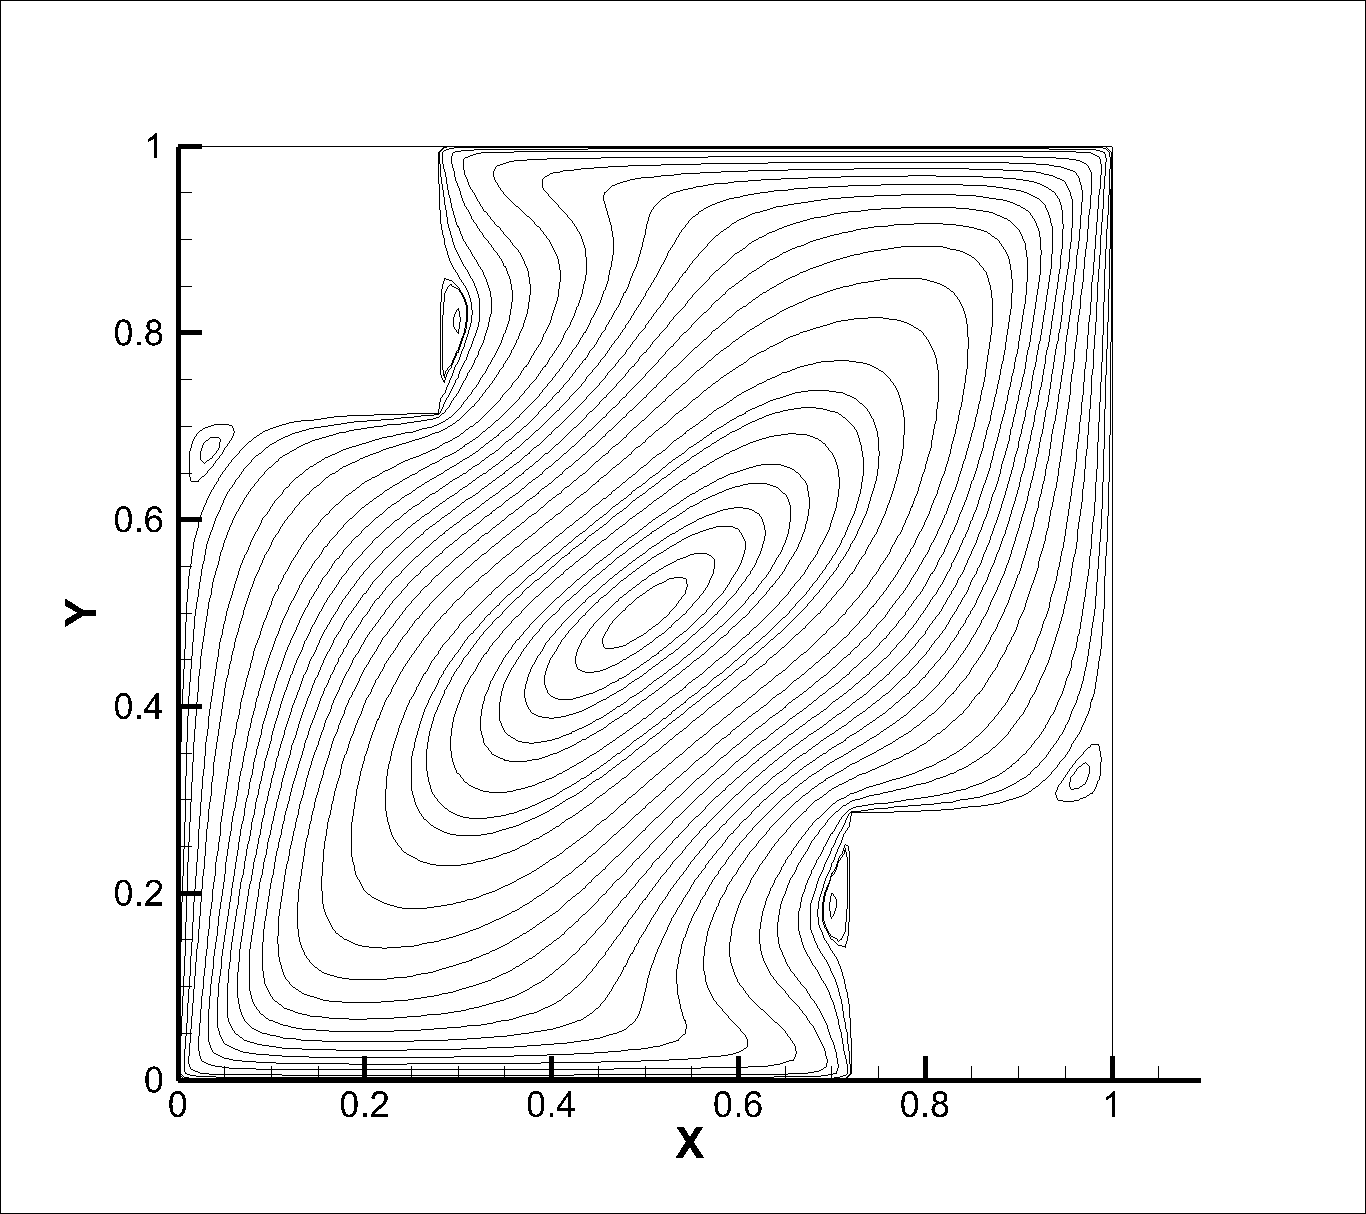
\includegraphics[width=0.25\textwidth]{images/stagerred/repsi400}
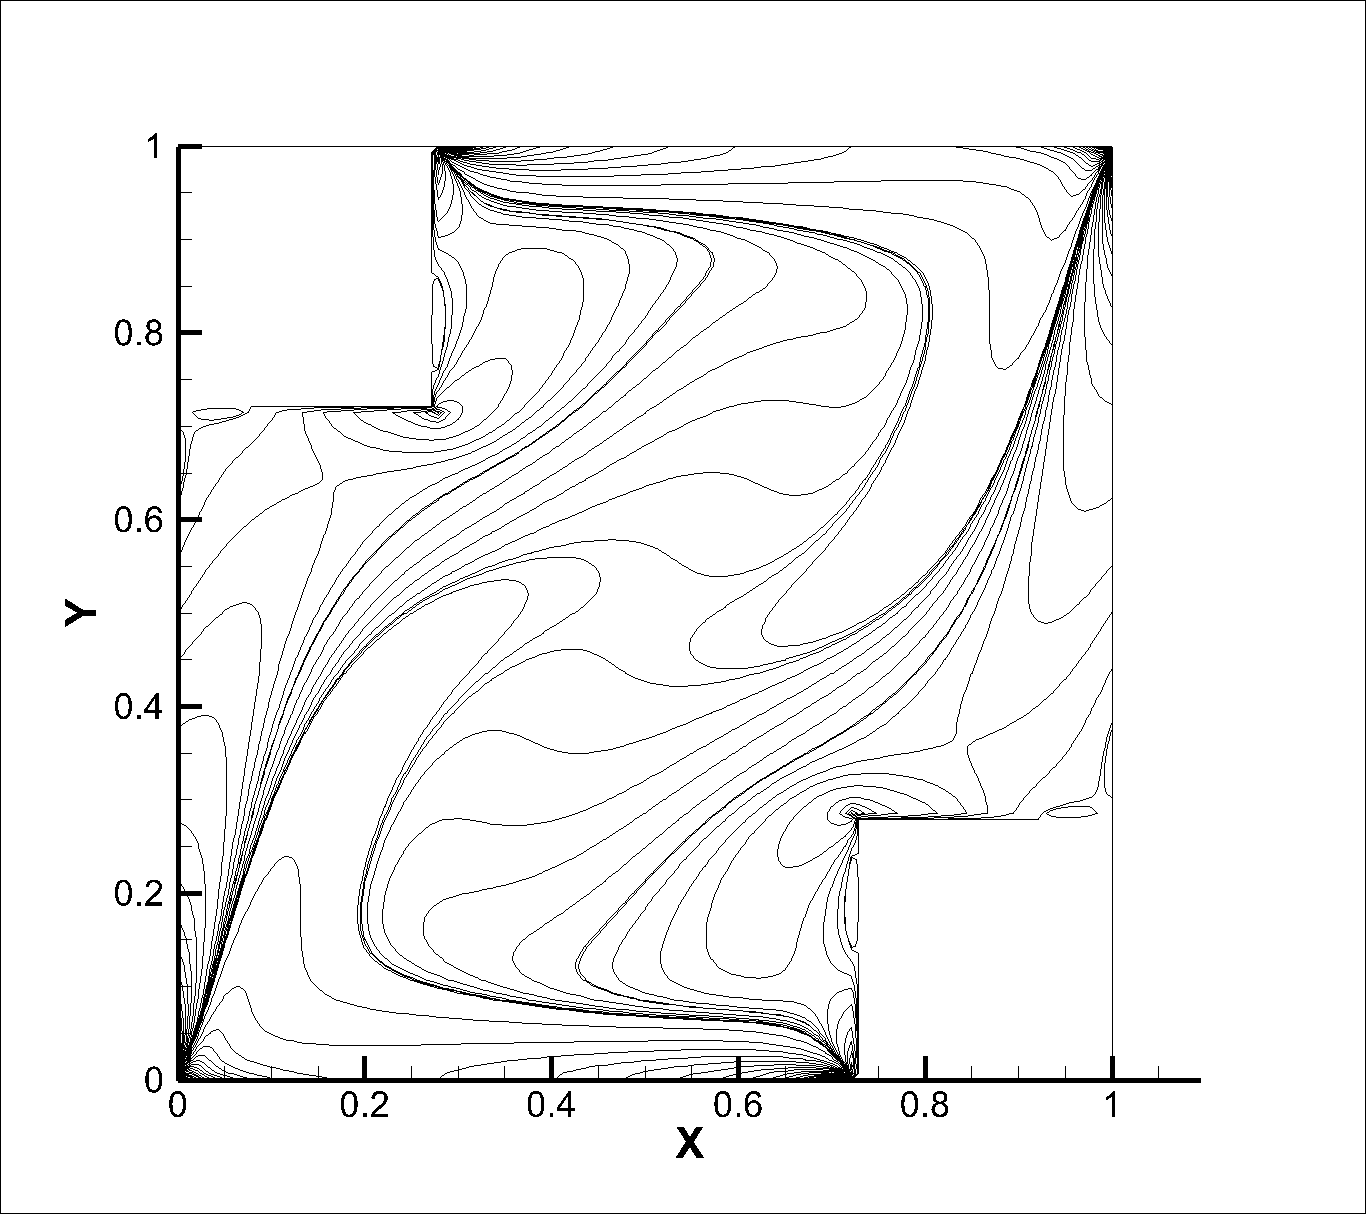
\includegraphics[width=0.25\textwidth]{images/stagerred/re400omega}
\caption{Streamlines and Vorticity plot in Staggered Cavity for Re 400. Results from Results from Zhou, et al [4] and Our results}
\end{figure}
\end{frame}

\begin{frame}{Results}{Staggered Cavity}
\begin{figure}[Hh]
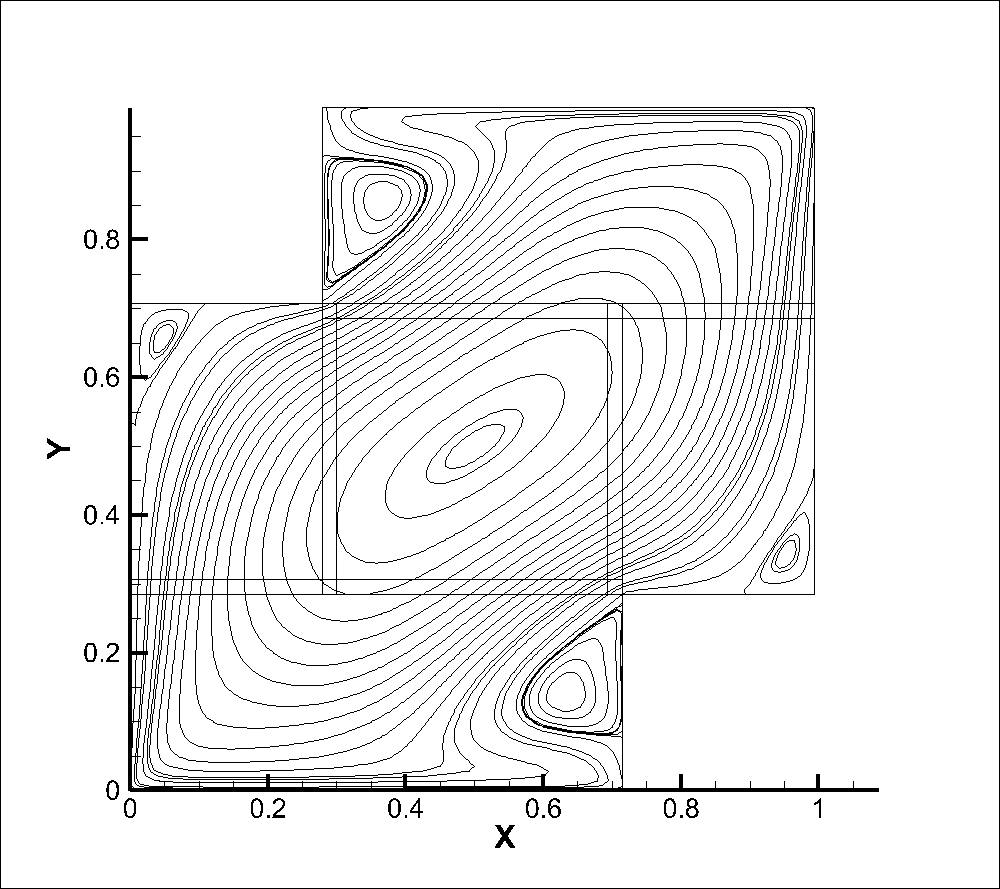
\includegraphics[width=0.49\textwidth]{images/stagerred/re1000psi}\hspace{1cm}
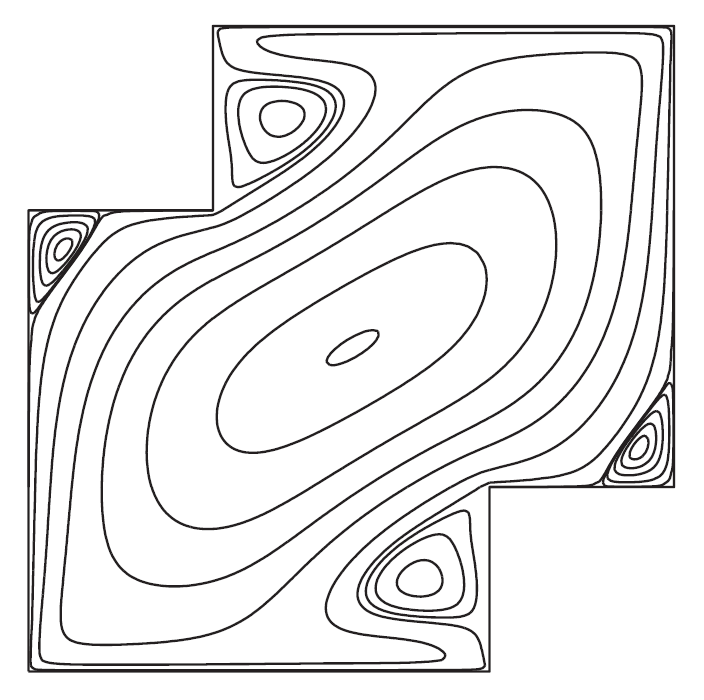
\includegraphics[width=0.39\textwidth]{images/stagerred/re1000psiN}
\caption{Streamlines plot at Re 1000. Our results vs Results from Zhou et al [4]}
\end{figure}
\end{frame}

\begin{frame}{Results}{Cross Cavity}
\textbf{Cross Cavity}\linebreak
\begin{figure}[H]
\centerline{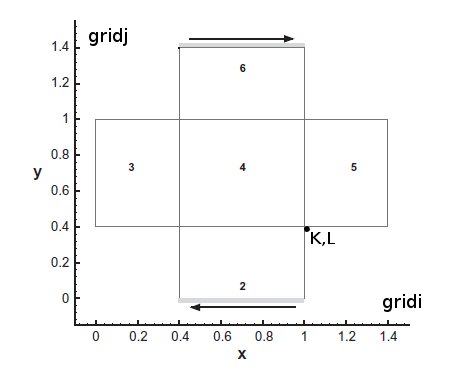
\includegraphics[width=0.4\textwidth]{images/jesus/domain}}
\caption{Problem domain of Cross Cavity.}
\end{figure}
\end{frame}


\begin{frame}{Results}{Cross Cavity}
Boundary conditions used to solve this domain is as follows,
\begin{eqnarray}
Left Wall:&
\omega_{0,j}=\frac{v_{0+1,j}-v_{0,j}}{\Delta x} \nonumber\\
& \omega_{gridi-k,j}=\frac{v_{gridi-k+1,j}-v_{gridi-k,j}}{\Delta x} \nonumber\\
Right Wall:&
\omega_{k-1,j}=\frac{v_{k-1,j}-v_{k-2,j}}{\Delta x} \nonumber\\
& \omega_{gridi-1,j}=\frac{v_{gridi-1+1,j}-v_{gridi-2,j}}{\Delta x} \nonumber\\
Bottom Wall:& 
\omega_{i,0}=-\frac{u_{i,1}-u_{i,0}}{\Delta y} \nonumber\\
& \omega_{i,l}=-\frac{u_{i,l+1}-u_{i,l}}{\Delta y} \nonumber\\
Top Wall:&
\omega_{i,gridj-l-1}=-\frac{u_{i,gridj-l-1}-u_{i,gridj-l-2}}{\Delta y} \nonumber\\
& \omega_{i,gridj-1}=-\frac{u_{i,gridj-1}-u_{i,gridj-2}}{\Delta y} \nonumber
\end{eqnarray}


\end{frame}


\begin{frame}{Results}{Cross Cavity}
\begin{figure}[hH]
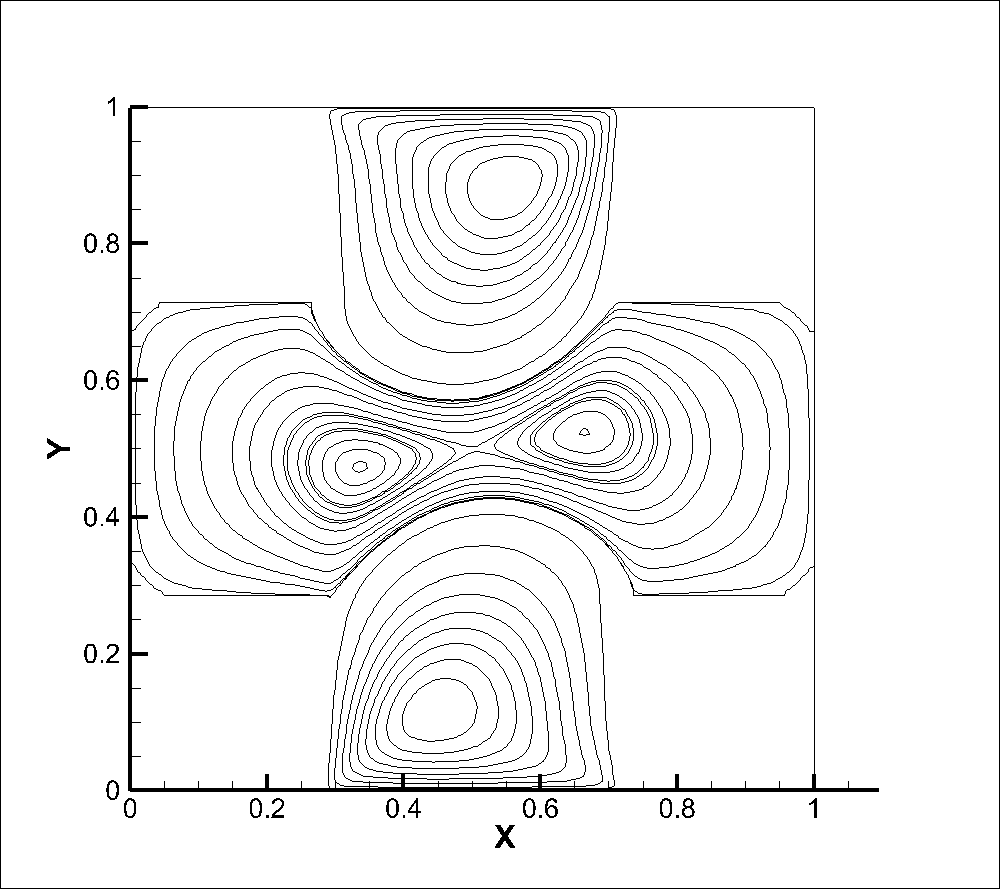
\includegraphics[width=0.25\textwidth]{images/jesus/re200psi}\hspace{1cm}
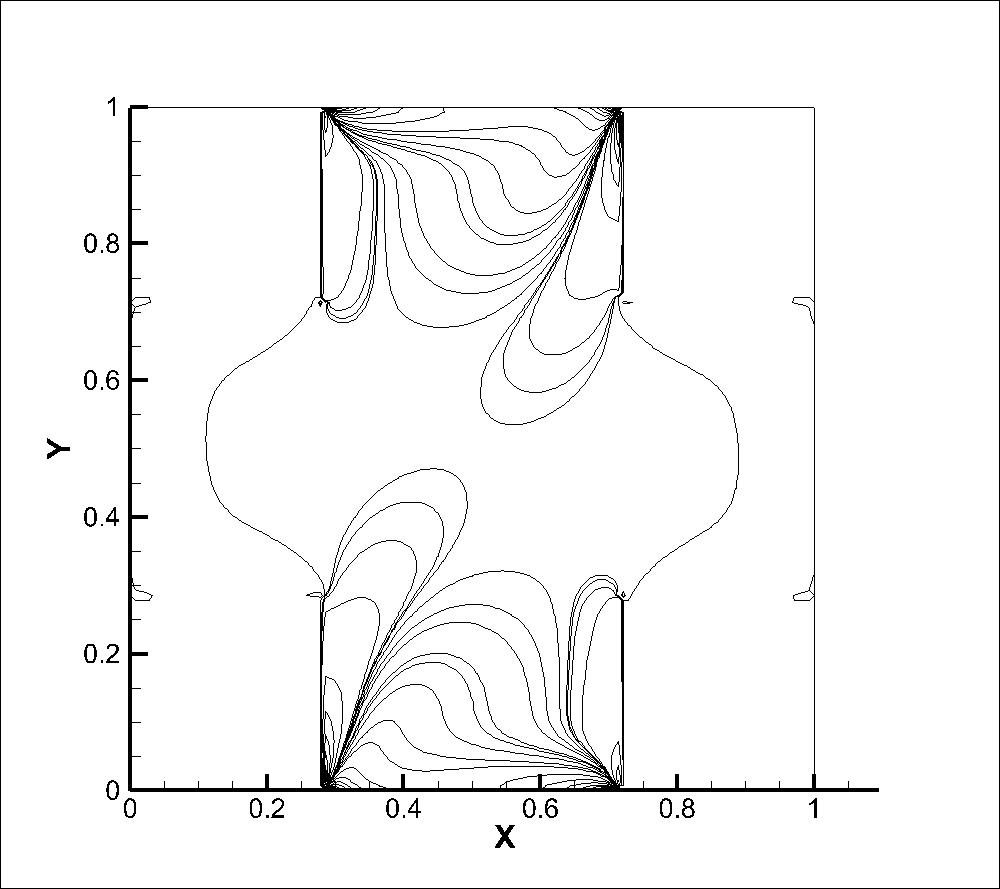
\includegraphics[width=0.25\textwidth]{images/jesus/re200omega}\\
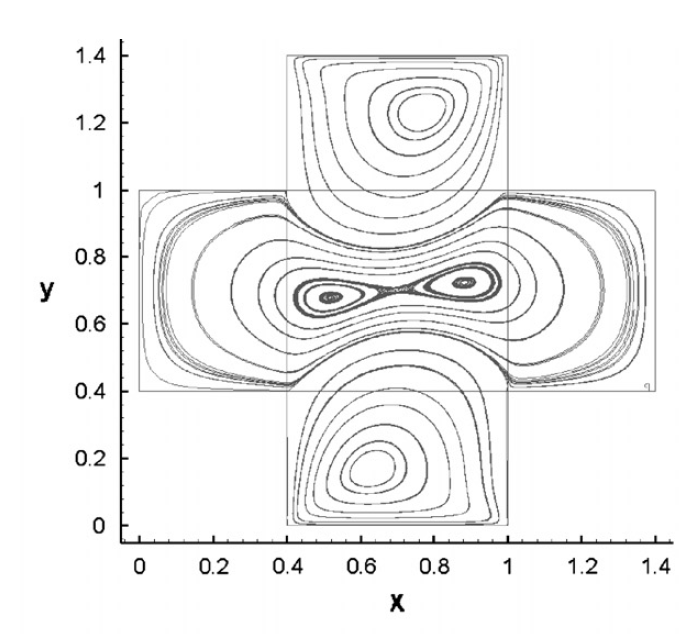
\includegraphics[width=0.25\textwidth]{images/jesus/re200psiP}\hspace{1cm}
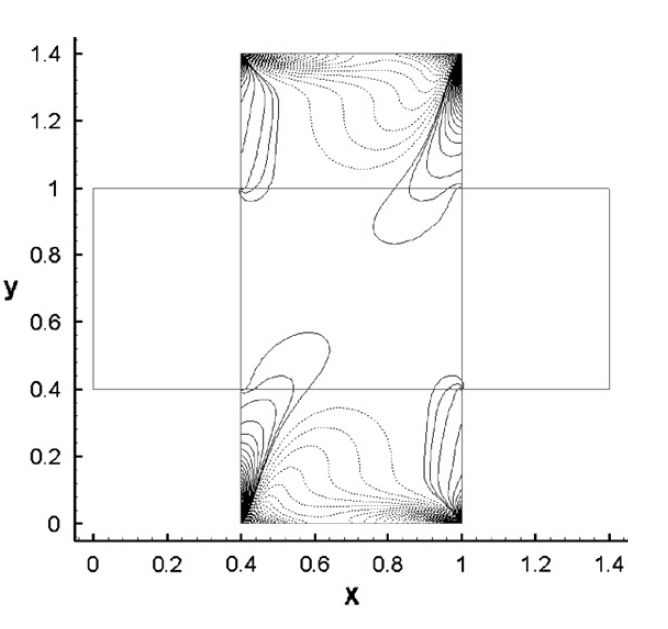
\includegraphics[width=0.25\textwidth]{images/jesus/re200omegaP}
\caption{Stream Lines and Vorticity plots in Cross Cavity. Our Results vs Results from De Vicente et al [5]}
\end{figure}
\end{frame}








\begin{frame}{Results}{Backward Facing Step Flow}
\textbf{Backward Facing Step Flow}\linebreak

\begin{figure}[hH]
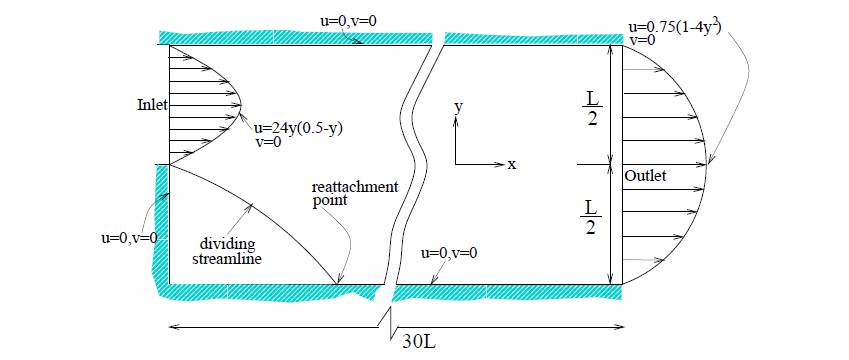
\includegraphics[width=0.5\textwidth]{images/l30l/domain}
\caption{Problem domain of the Backward step flow.}
\end{figure}
In this problem fluid enters the domain with the parabolic profile into a larger cross-section area tube. The outlet conditions correspond to fully developed flow.
\end{frame}


\begin{frame}{Results}{Backward Facing Step Flow}
These Boundary conditions are as follows,
\begin{eqnarray}
TOP &:& u = v = \omega = 0; \psi =0.5 \nonumber\\
BOTTOM &:& u = v = \psi = \omega= 0 \nonumber\\
INLET &:&  u = v = \psi = \omega= 0  \hspace{1cm} \nonumber\\
&& at -0.5 \leq y \leq 0 \nonumber\\
&& u=12y(1-2y), v=0, \psi = 2y^{2}(3-4y), \omega = 12(4y-1) \nonumber\\
&& at 0 \leq y \leq 0.5 \nonumber\\
OUTLET &:& u=\frac{3}{4}(1-4y^{2}), v=0, \psi = \frac{1}{4}(1+3y-4y^{3}), \omega = 6y \nonumber
\end{eqnarray}
\end{frame}

\begin{frame}{Results}{Backward Facing Step Flow}
\begin{figure}[hH]
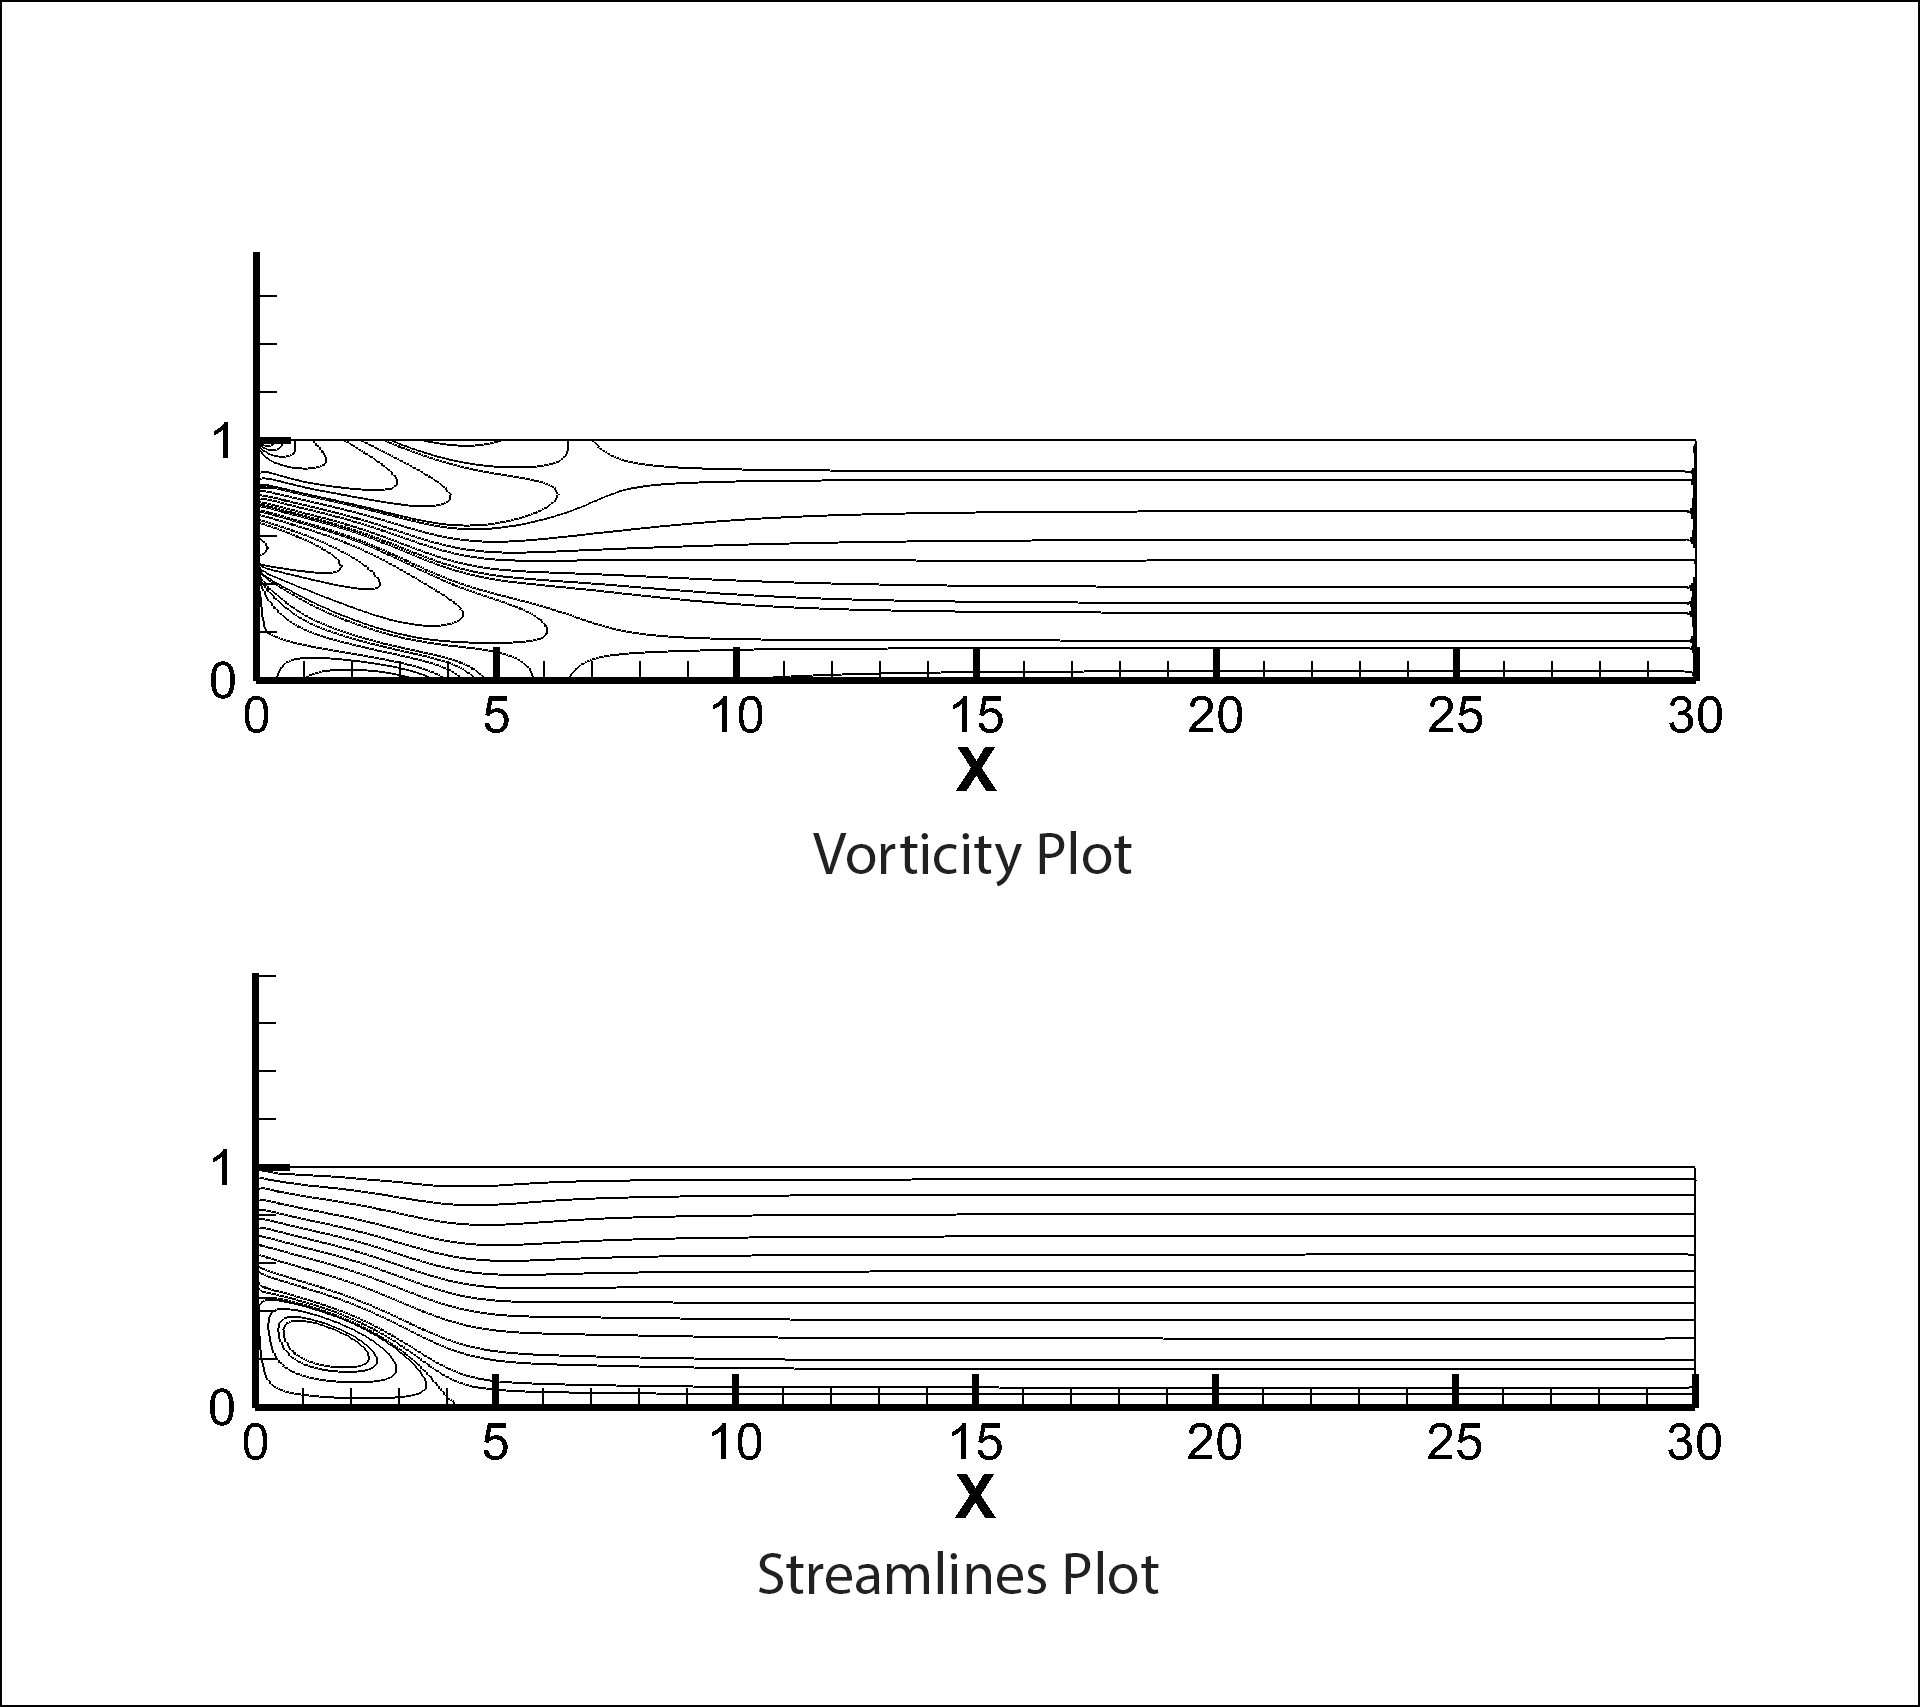
\includegraphics[width=0.40\textwidth]{images/l30l/our400}
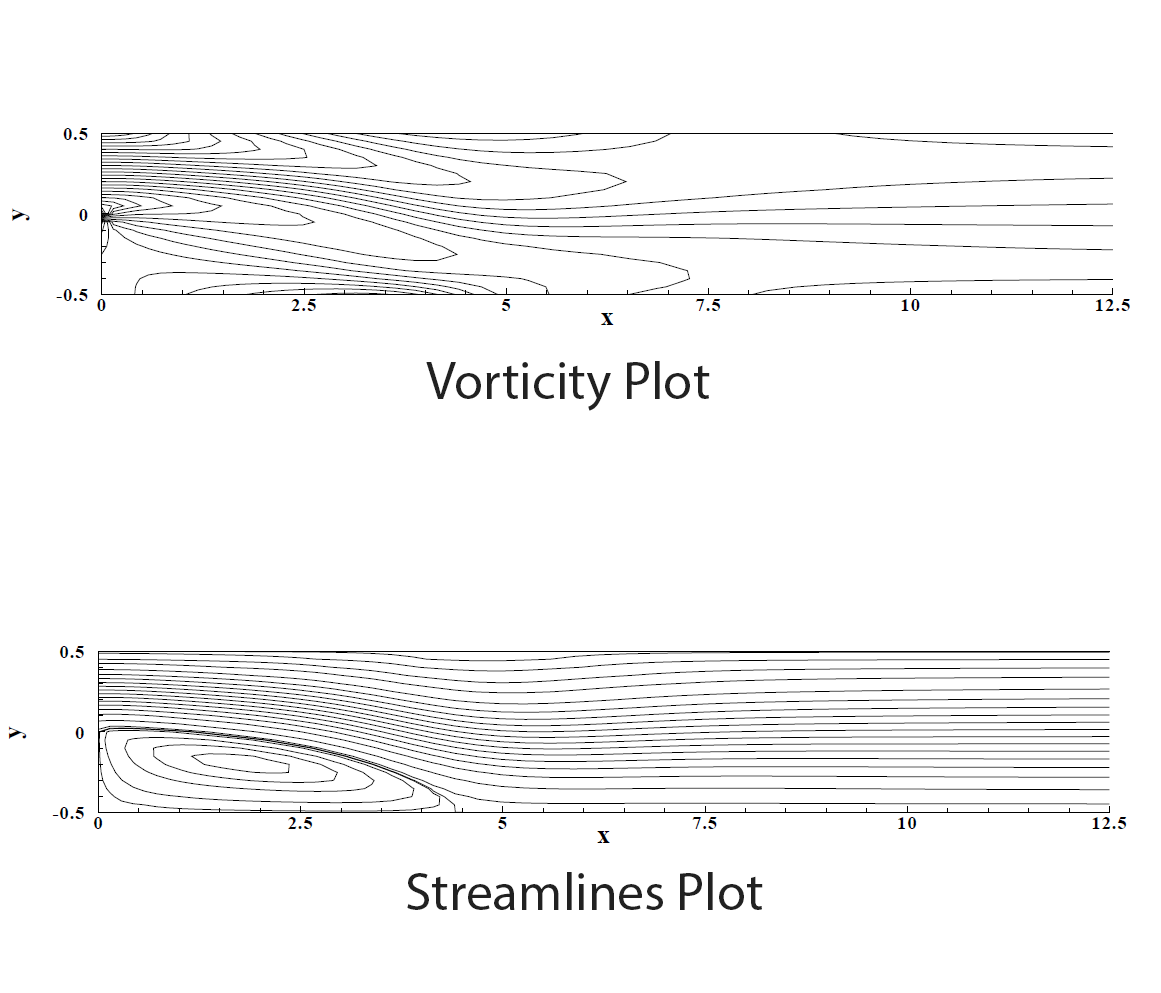
\includegraphics[width=0.40\textwidth]{images/l30l/sir400}
\caption{Streamlines and Vorticity Plot. Our Results vs Dr. Jiten Kalita's thesis [3] at Re 400}
\end{figure}
\end{frame}


\begin{frame}{Results}{Backward Facing Step Flow}
\begin{figure}[hH]
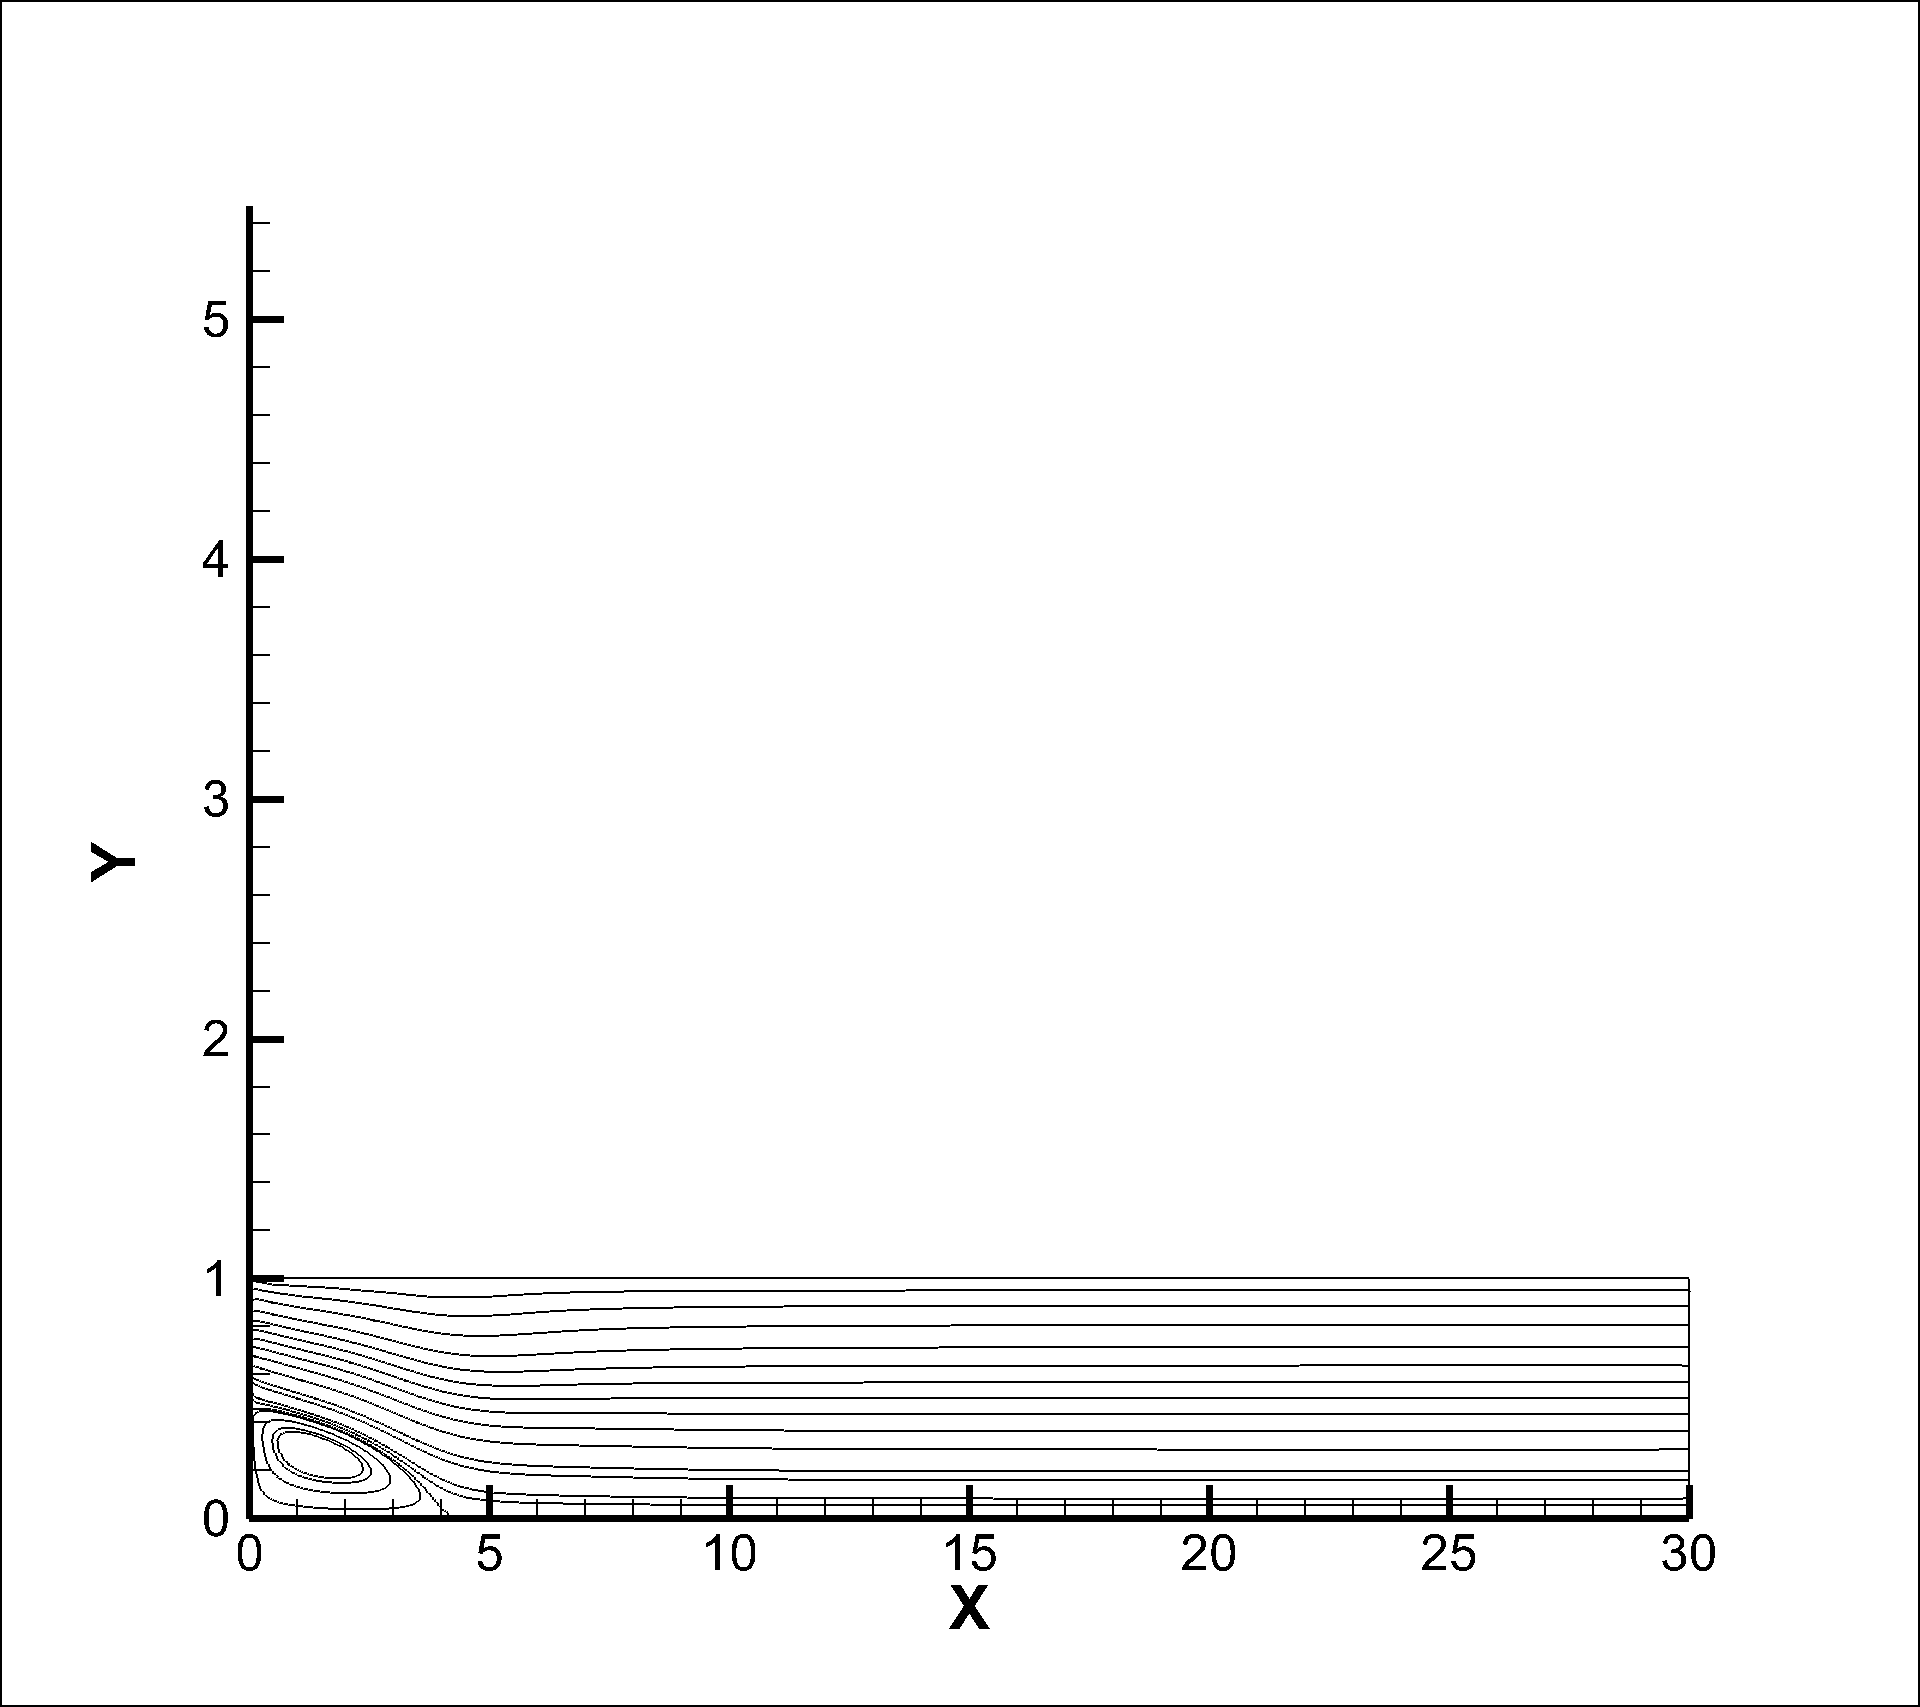
\includegraphics[width=0.25\textwidth]{figures/l30l/400psi}
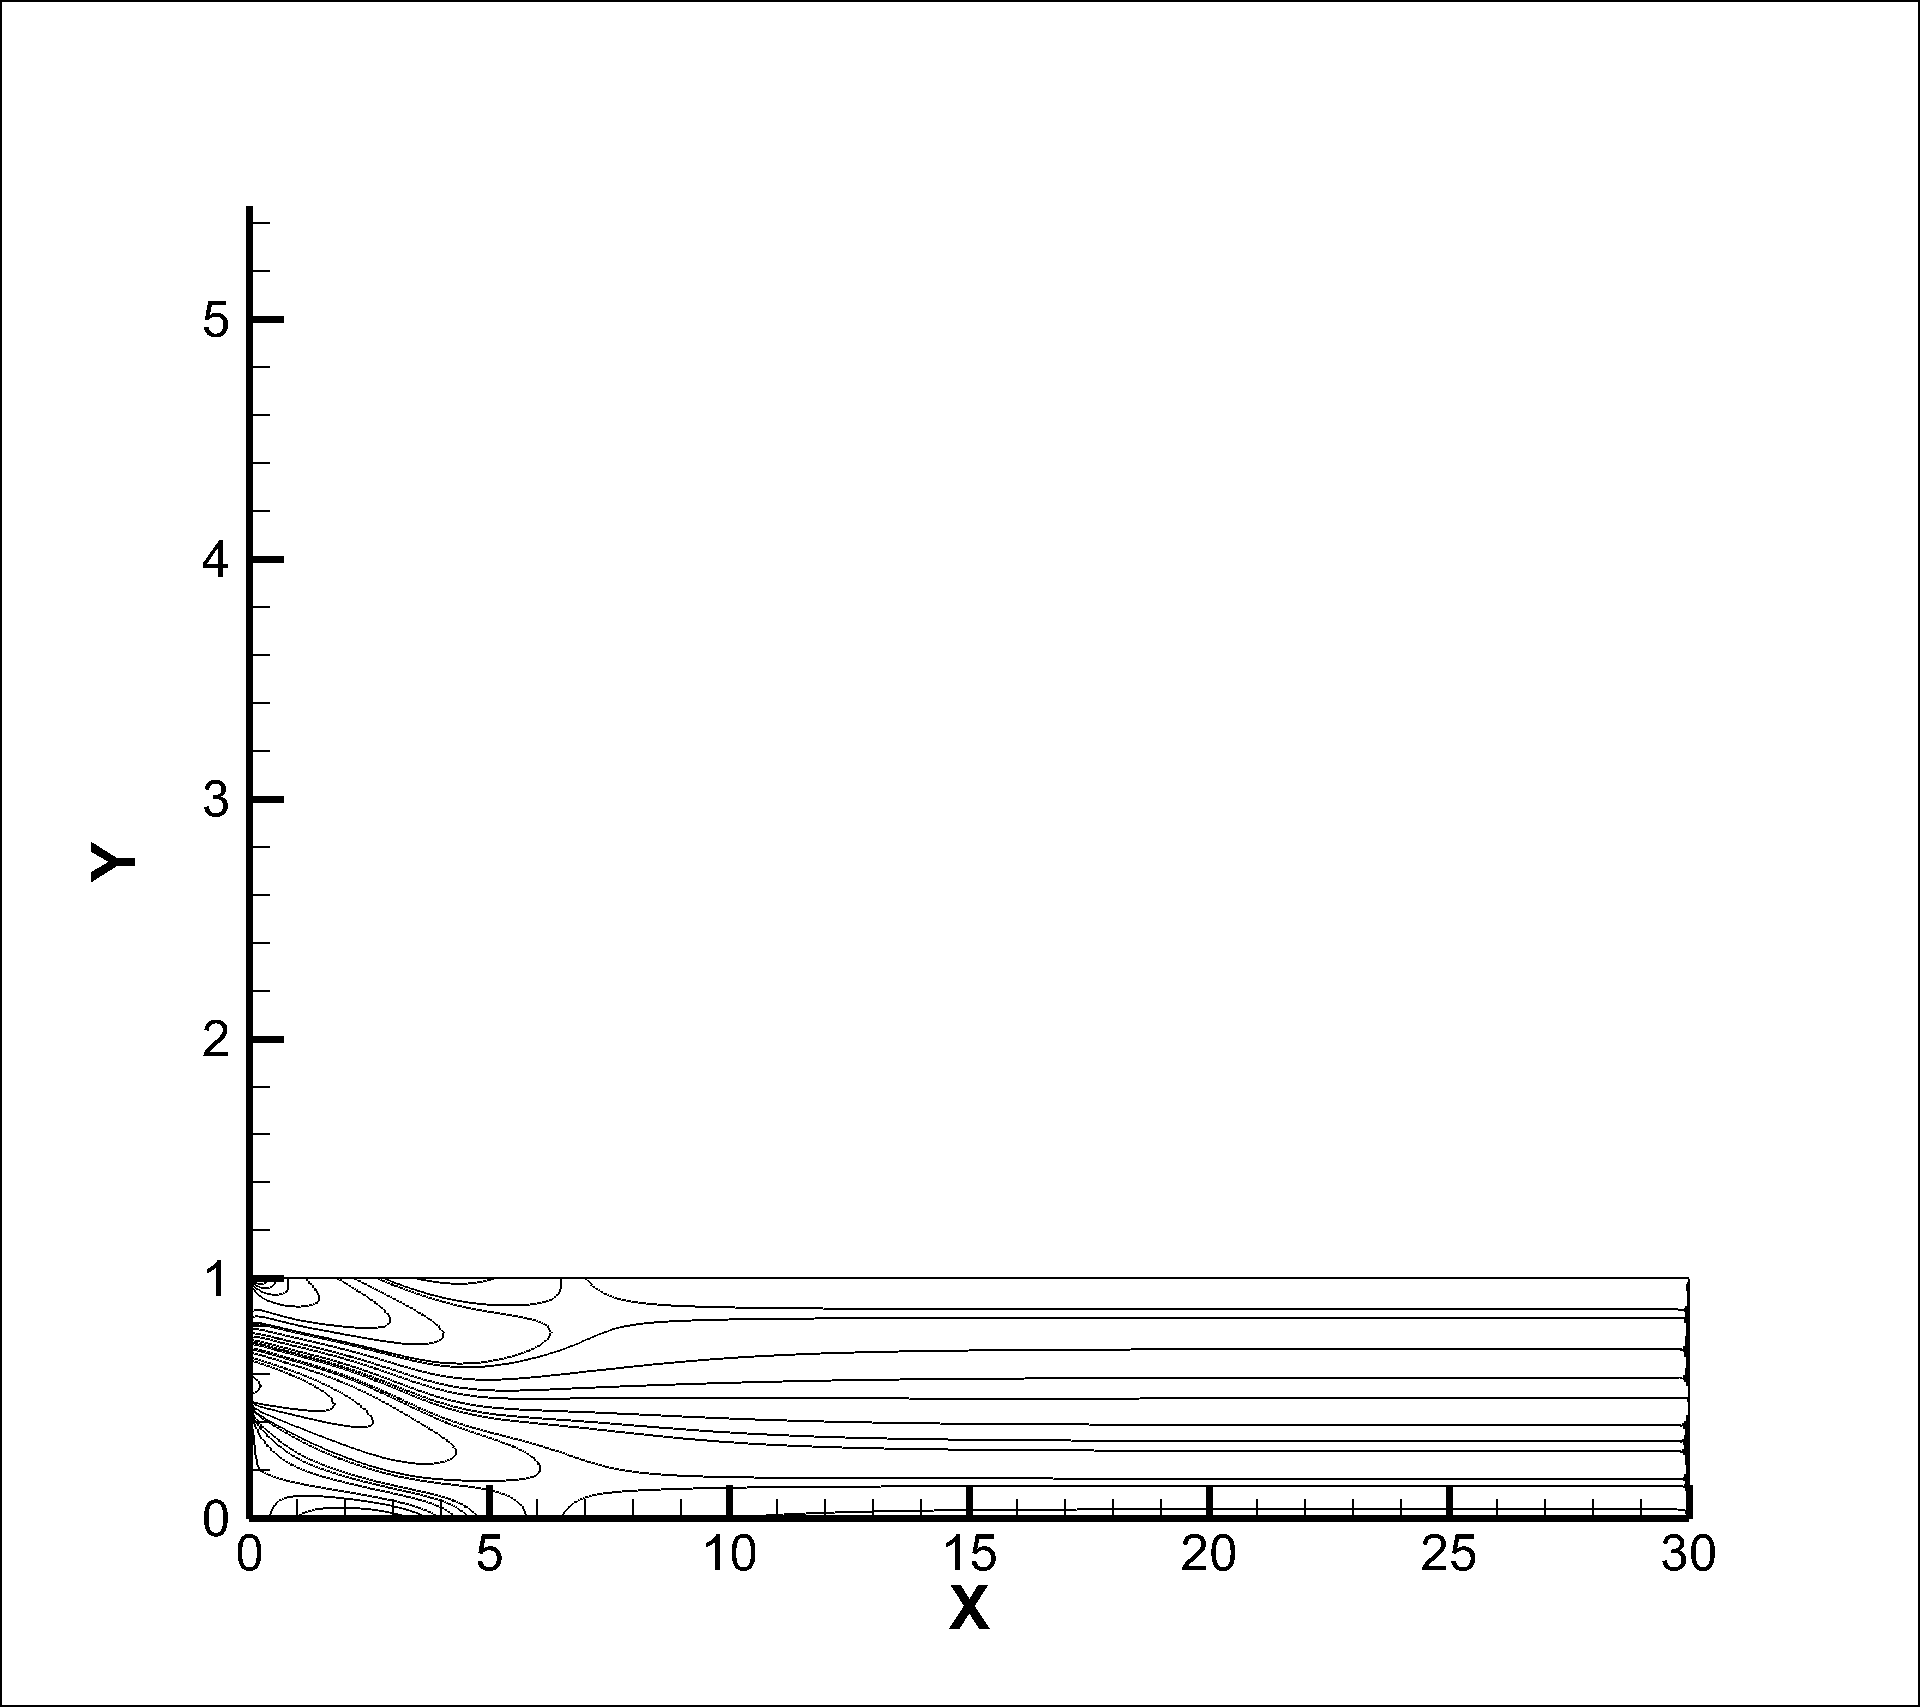
\includegraphics[width=0.25\textwidth]{figures/l30l/400omega}
\caption{Plots at Reynolds number 400. Stream Lines and Vorticity plots calculated.}
\end{figure}
\begin{figure}[hH]
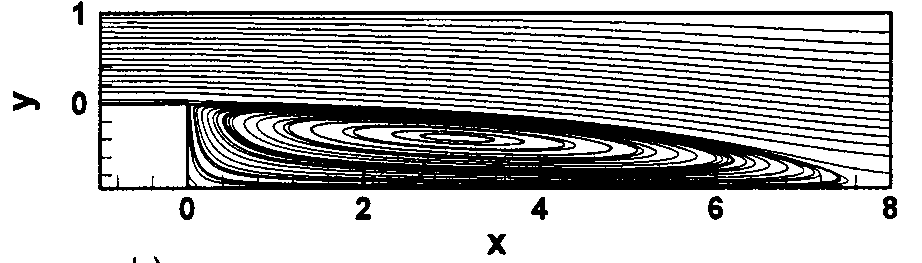
\includegraphics[width=0.5\textwidth]{figures/sir/re400psi}
\caption{Stream Lines plot from G.Biswas et. al.}
\end{figure}
\end{frame}

\begin{frame}{Results}{Backward Facing Step Flow}
\begin{figure}[hH]
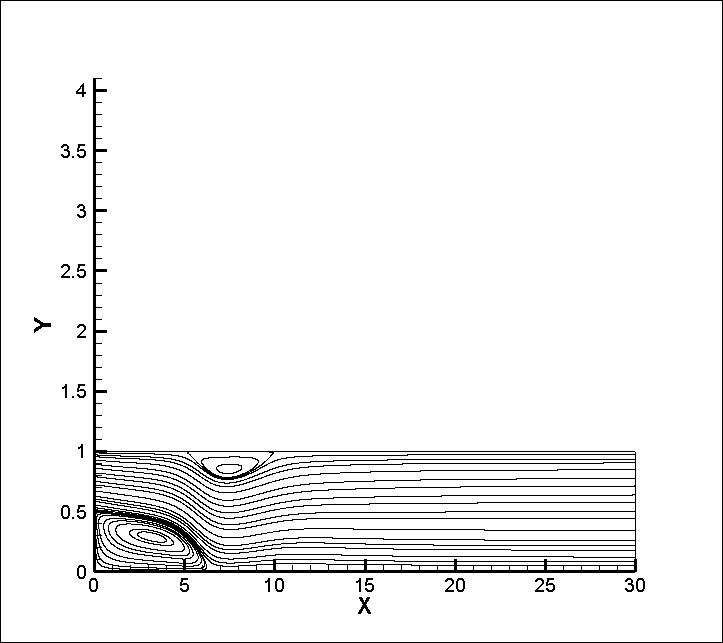
\includegraphics[width=0.25\textwidth]{figures/cuda/psi}
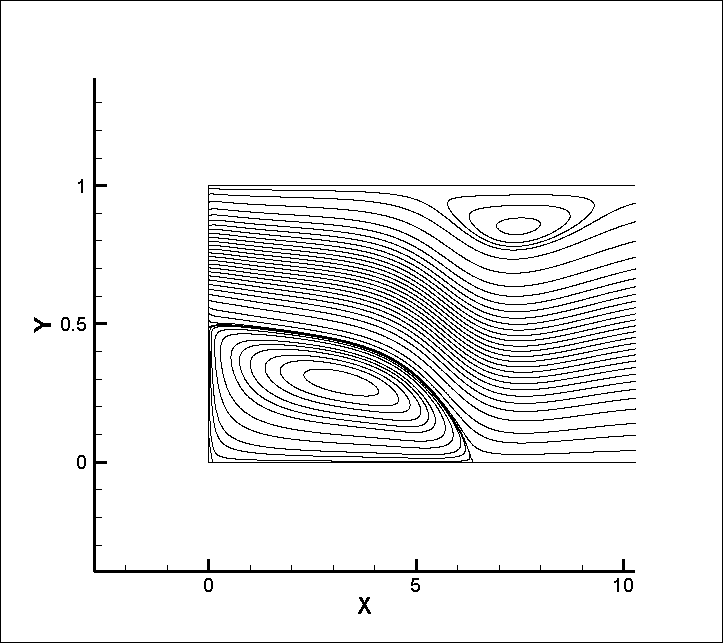
\includegraphics[width=0.25\textwidth]{figures/cuda/psizoom}
\caption{Stream Lines and Vorticity plots at Reynolds number 800 on grid size 150x4500. Expansion ratio H/h = 0.15.}
\end{figure}
The above results were obtained at Reynolds number 800 using grid size
150x4500. The code was simulated till error 0.001 on CUDA program.
\end{frame}

\begin{frame}{Results}{Backward Facing Step Flow}
\begin{figure}[hH]
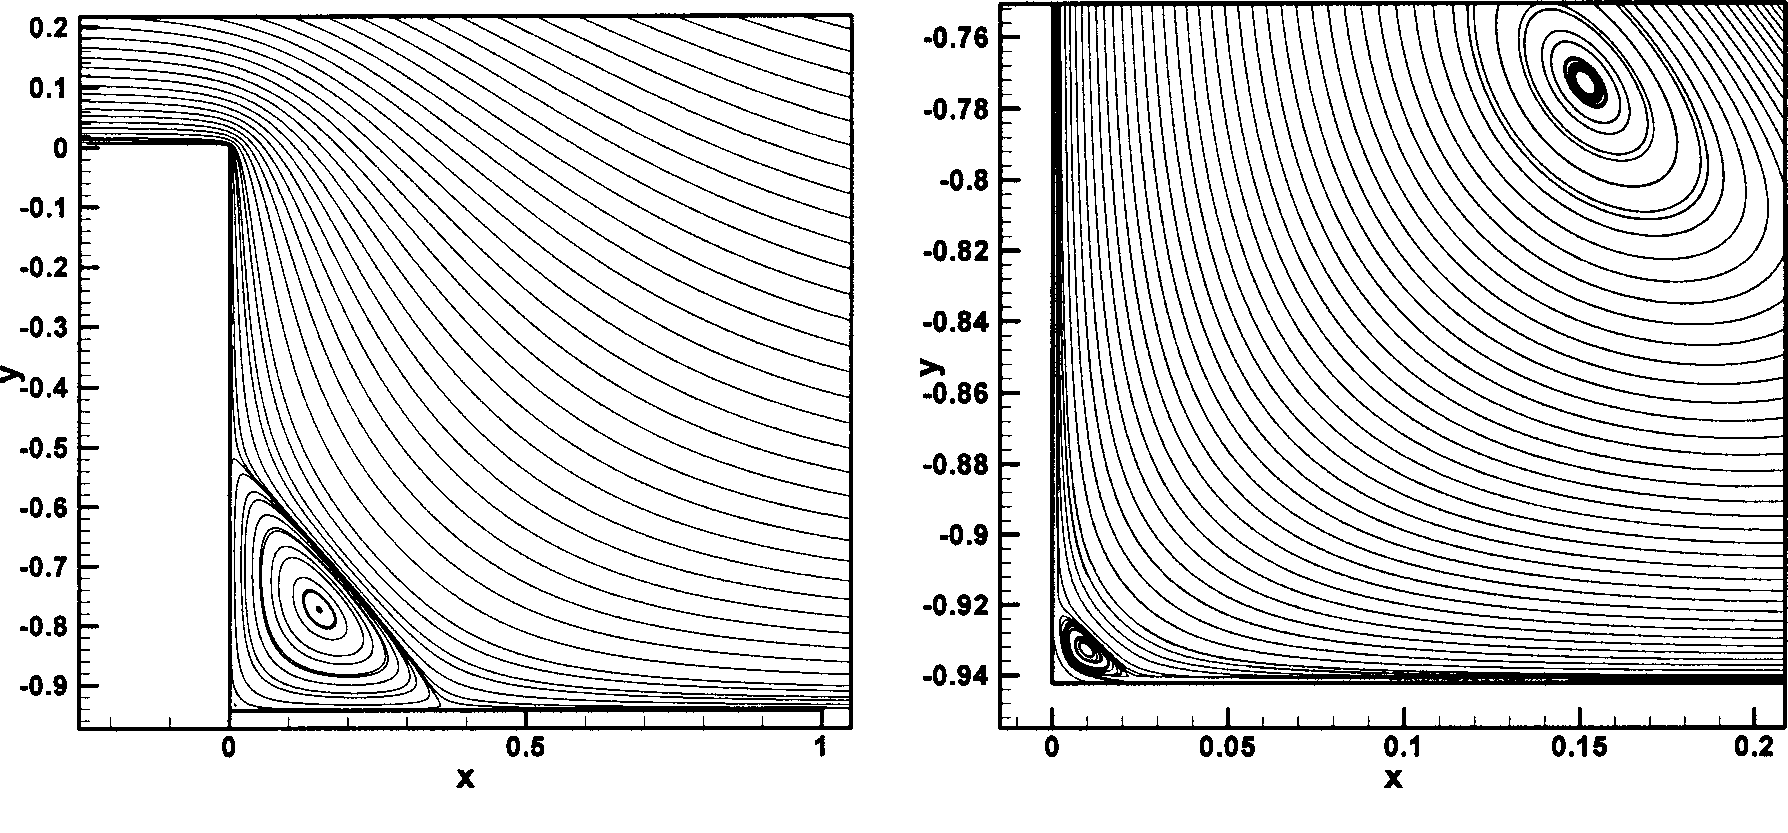
\includegraphics[width=0.5\textwidth]{figures/sir/re1vertex}

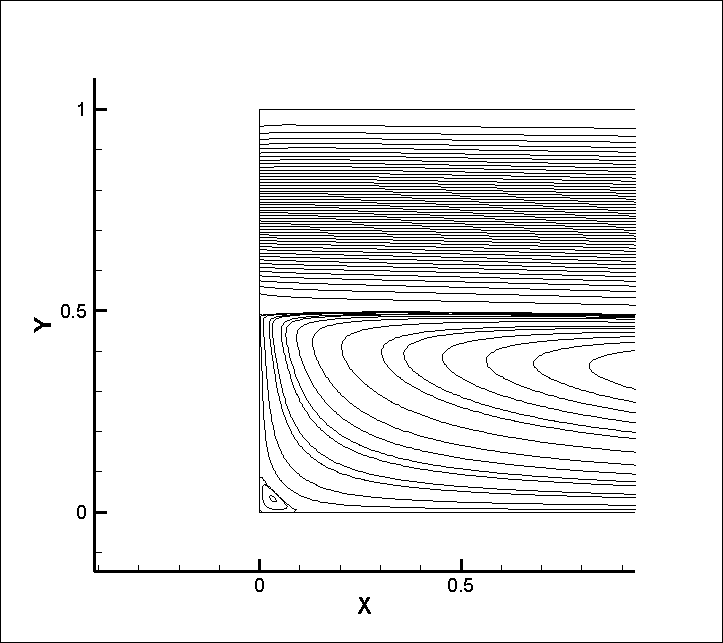
\includegraphics[width=0.25\textwidth]{figures/cuda/psizoom1}
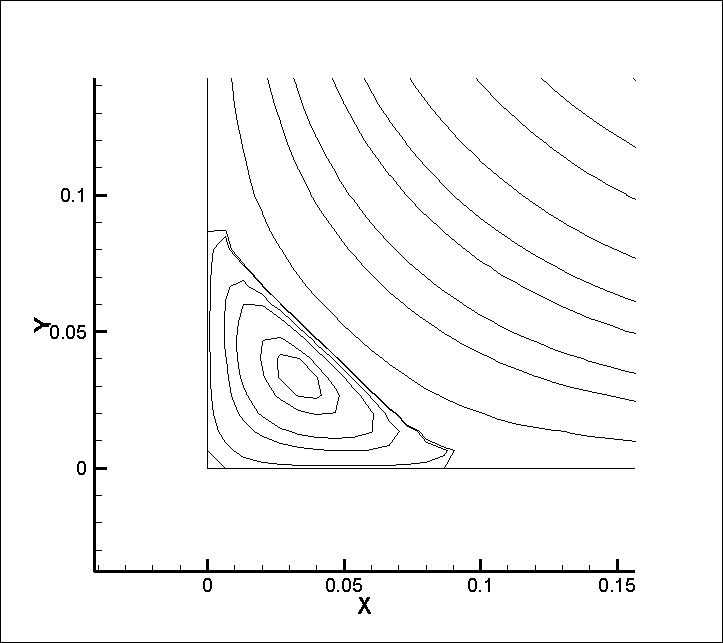
\includegraphics[width=0.25\textwidth]{figures/cuda/psizoom2}
\caption{a).Stream Lines and its further zoom. Plots at Re=1 from G. Biswas et.al. b).Plots calculated at Re=800.}
\end{figure}
\end{frame}


\begin{frame}{Conclusion}
\begin{itemize}
\item CUDA  allowed to go to higher grid size which was previously not possible with serial code. 
\item  CUDA computation is alot faster and efficient than average serial codes for simulation and other renderings hence it would be very useful in Direct Numerical Simulation.

\end{itemize}

\end{frame}









\begin{frame}{Bibliography}
[1]	Ghia, Urmila, Kirti N. Ghia, and C. T. Shin. "High-Re solutions for incompressible flow 	using the Navier-Stokes equations and a multigrid method." Journal of 	computational physics 48.3 (1982): 387-411.\linebreak

[2]	Poochinapan, Kanyuta. "Numerical Implementations for 2D Lid-Driven Cavity Flow in 	Stream Function Formulation." ISRN Applied Mathematics 2012 (2012).\linebreak

[3]	Dr. Jiten C. Kalita, "HOC Schemes for incompressible viscous flows: Application and 	Development". Department of Mathematics, Indian Institute of Technology Guwahati (2002).\linebreak

[4]	Zhou, Y. C., et al. "DSC solution for flow in a staggered double lid driven cavity." 	International Journal for Numerical Methods in Engineering 57.2 (2003): 211-234.
\end{frame}
\begin{frame}{Bibliography}
[5]	De Vicente, Javier, et al. "Stability analysis in spanwise-periodic double-sided lid-	driven cavity flows with complex cross-sectional profiles." Computers \& Fluids 43.1 	(2011): 143-153.\linebreak

[6] G Biswas, M Breuer, and F Durst. Backward-facing step flows for various expansion ratios at low and moderate reynolds numbers. Journal of fluids engineering, 126(3):362–374, 2004.\linebreak

[7] Thibault, Julien C., and Inanc Senocak. "CUDA implementation of a Navier-Stokes solver on multi-GPU desktop platforms for incompressible flows." Proceedings of the 47th AIAA Aerospace Sciences Meeting. 2009.
\end{frame}

\end{document}